%\renewcommand{\theequation}{\theenumi}
%\begin{enumerate}[label=\arabic*.,ref=\thesubsection.\theenumi]
%\numberwithin{equation}{enumi}
%
%
\item Check which of the following are solutions of the equation 
%
\begin{align}
\myvec{1 & -2}\vec{x} &= 4
\end{align}
%
%
\begin{enumerate}[itemsep=2pt]
\begin{multicols}{2}
\item $\myvec{0 \\ 2}$
\item $\myvec{2 \\ 0}$
\item $\myvec{4 \\ 0}$
\item $\myvec{\sqrt{2} \\ 4\sqrt{2}}$
\item $\myvec{1 \\ 1}$
\end{multicols}
\end{enumerate}
%
\solution

\begin{table}[!ht]
\centering
\resizebox{\columnwidth}{!}{\begin{tabular}{|c|c|c|c|} 
\hline
kind of  cake & No.of cakes & Flour& Fat\\
\hline
1st & x & 200g  &  25g \\ 
\hline
2nd& y& 100g&  50g  \\ 
\hline
Total& x+y& 5 kg=5000g&1kg=1000g \\ 
\hline
\end{tabular}}
\caption{Ingredients used in making the cake is flour and fat }
\label{opt/13/tab:table1}
\end{table}
Let the  1st kind  be $x$ and the 2nd kind be $y$  such that 
\begin{align}
x \geq 0 \\
y \geq 0 
\end{align}
According to the question,
\begin{align}
2{x} + {y} \leq 50
\\
{x} + 2{y} \leq 40
\end{align}
$\therefore$ Our problem is
\begin{align}
\max_{\vec{x}} Z &= \myvec{1& 1}\vec{x}\\
s.t. \quad \myvec{2 & 1 \\ 1& 2}\vec{x} &\preceq \myvec{50\\40} 
\end{align}
Lagrangian function is given by
\begin{equation}
\begin{aligned}
&L(\vec{x},\boldsymbol{\lambda}) \\ &= \myvec{1 & 1}\vec{x}+\lcbrak{\sbrak{\myvec{2 & 1}\vec{x}-50}} \\ &+ \sbrak{\myvec{1 & 2}\vec{x}-40}\\ &+ \sbrak{\myvec{-1 & 0}\vec{x}} +\rcbrak{\sbrak{\myvec{0 & -1}\vec{x}}}\boldsymbol{\lambda}
\end{aligned}
\end{equation}
where,
\begin{align}
\boldsymbol{\lambda} &= \myvec{\lambda_1 \\ \lambda_2 \\ \lambda_3 \\ \lambda_4 \\ \lambda_5 \\ \lambda_6}
\end{align}
Now,
\begin{align}
\nabla L(\vec{x},\boldsymbol{\lambda}) &= \myvec{1+ \myvec{2 & 1 & -1 & 0 }\boldsymbol{\lambda}\\ 1+\myvec{1 & 2 & 0 & -1}\boldsymbol{\lambda} \\ \myvec{2 & 1}\vec{x}-50\\ \myvec{1& 2}\vec{x}-40 \\  \myvec{-1 & 0}\vec{x} \\ \myvec{0 & -1}\vec{x}}
\end{align}
$\therefore$ Lagrangian matrix is given by
\begin{align}
\myvec{0 & 0 & 2 & 1& -1 & 0 \\ 0 & 0 & 1 & 2  & 0 & -1 \\ 2 & 1 & 0 & 0 & 0 & 0 \\ 1 & 2 & 0 & 0 & 0 & 0  \\ -1 & 0 & 0 & 0 & 0 & 0  \\ 0 & -1 & 0 & 0 & 0 & 0 }\myvec{\vec{x} \\ \boldsymbol{\lambda} } &= \myvec{-1 \\ -1 \\ 50\\ 4 0\\ 0 \\0 }
\end{align}
Considering $\lambda_1,\lambda_2$ as only active multiplier,
\begin{align}
\myvec{0 & 0 & 2 & 1 \\ 0 & 0 & 1 & 2 \\ 2 & 1 & 0 & 0 \\ 1 & 2 & 0 & 0}\myvec{\vec{x}\\ \boldsymbol{\lambda}} &= \myvec{-1 \\ -1 \\ 5 0\\ 40}
\end{align}
resulting in,
\begin{align}
\myvec{\vec{x} \\ \boldsymbol{\lambda}} &= \myvec{0 & 0 & 2 & 1 \\ 0 & 0 & 1 & 2 \\ 2 & 1 & 0 & 0 \\ 1& 2 & 0 & 0}^{-1}\myvec{-1 \\ -1 \\ 50 \\ 40}
\\
\implies   \myvec{\vec{x} \\ \boldsymbol{\lambda}} &= \myvec{0 & 0 & \frac{2}{3} & \frac{-1}{3} \\ 0 & 0 & \frac{-1}{3} & \frac{2}{3} \\ \frac{2}{3} & \frac{-1}{3} & 0 & 0 \\ \frac{-1}{3} & \frac{2}{3} & 0 & 0}\myvec{-1 \\ -1 \\ 50 \\ 40}
\\
\implies \myvec{\vec{x} \\ \boldsymbol{\lambda}} &= \myvec{20 \\ 10 \\ -0.3 \\ -0.3 }
\end{align}
$\because \boldsymbol{\lambda}=\myvec{-0.3 \\ -0.3} \succ \vec{0} $
\\
$\therefore$ Optimal solution is given by
\begin{align}
    \vec{x} &= \myvec{20\\10} \\
    Z &= \myvec{1& 1}\vec{x} \\
    &= \myvec{1 & 1}\myvec{20 \\ 10} \\
    &= 60
\end{align}
By using cvxpy in python ,
\begin{align}
    \vec{x}=\myvec{20\\10}\\
    Z = 60
\end{align}
Hence No.of cakes \boxed{x=20} 1st kind and  .of cakes \boxed{y=10} 2nd kind should be used to maximum No. of cakes \boxed{Z=60}.  This is
verified in Fig. \ref{opt/13/fig: Graphical Solution}.	
%
\begin{figure}[!ht]
\centering
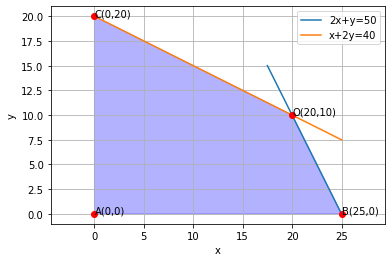
\includegraphics[width=\columnwidth]{solutions/su2021/2/13/Figure9.png}
\caption{Graphical Solution}
\label{opt/13/fig: Graphical Solution}	
\end{figure}

\item Find the value of $k$, if $\myvec{2\\1}$ is a solution of the equation 
%
\\
\solution
\documentclass[journal,12pt,twocolumn]{IEEEtran}

\usepackage{setspace}
\usepackage{gensymb}

\singlespacing


\usepackage[cmex10]{amsmath}

\usepackage{amsthm}

\usepackage{mathrsfs}
\usepackage{txfonts}
\usepackage{stfloats}
\usepackage{bm}
\usepackage{cite}
\usepackage{cases}
\usepackage{subfig}

\usepackage{longtable}
\usepackage{multirow}

\usepackage{enumitem}
\usepackage{mathtools}
%\usepackage{steinmetz}
\usepackage{tikz}
\usepackage{circuitikz}
\usepackage{verbatim}
%\usepackage{tfrupee}
\usepackage[breaklinks=true]{hyperref}

\usepackage{tkz-euclide}

\usetikzlibrary{calc,math}
\usepackage{listings}
    \usepackage{color}                                            %%
    \usepackage{array}                                            %%
    \usepackage{longtable}                                        %%
    \usepackage{calc}                                             %%
    \usepackage{multirow}                                         %%
    \usepackage{hhline}                                           %%
    \usepackage{ifthen}                                           %%
    \usepackage{lscape}     
\usepackage{multicol}
\usepackage{chngcntr}

\DeclareMathOperator*{\Res}{Res}

\renewcommand\thesection{\arabic{section}}
\renewcommand\thesubsection{\thesection.\arabic{subsection}}
\renewcommand\thesubsubsection{\thesubsection.\arabic{subsubsection}}

\renewcommand\thesectiondis{\arabic{section}}
\renewcommand\thesubsectiondis{\thesectiondis.\arabic{subsection}}
\renewcommand\thesubsubsectiondis{\thesubsectiondis.\arabic{subsubsection}}


\hyphenation{op-tical net-works semi-conduc-tor}
\def\inputGnumericTable{}                                 %%

\lstset{
%language=C,
frame=single, 
breaklines=true,
columns=fullflexible
}
\begin{document}


\newtheorem{theorem}{Theorem}[section]
\newtheorem{problem}{Problem}
\newtheorem{proposition}{Proposition}[section]
\newtheorem{lemma}{Lemma}[section]
\newtheorem{corollary}[theorem]{Corollary}
\newtheorem{example}{Example}[section]
\newtheorem{definition}[problem]{Definition}

\newcommand{\BEQA}{\begin{eqnarray}}
\newcommand{\EEQA}{\end{eqnarray}}
\newcommand{\define}{\stackrel{\triangle}{=}}
\bibliographystyle{IEEEtran}
\providecommand{\mbf}{\mathbf}
\providecommand{\pr}[1]{\ensuremath{\Pr\left(#1\right)}}
\providecommand{\qfunc}[1]{\ensuremath{Q\left(#1\right)}}
\providecommand{\sbrak}[1]{\ensuremath{{}\left[#1\right]}}
\providecommand{\lsbrak}[1]{\ensuremath{{}\left[#1\right.}}
\providecommand{\rsbrak}[1]{\ensuremath{{}\left.#1\right]}}
\providecommand{\brak}[1]{\ensuremath{\left(#1\right)}}
\providecommand{\lbrak}[1]{\ensuremath{\left(#1\right.}}
\providecommand{\rbrak}[1]{\ensuremath{\left.#1\right)}}
\providecommand{\cbrak}[1]{\ensuremath{\left\{#1\right\}}}
\providecommand{\lcbrak}[1]{\ensuremath{\left\{#1\right.}}
\providecommand{\rcbrak}[1]{\ensuremath{\left.#1\right\}}}
\theoremstyle{remark}
\newtheorem{rem}{Remark}
\newcommand{\sgn}{\mathop{\mathrm{sgn}}}
\providecommand{\abs}[1]{\left\vert#1\right\vert}
\providecommand{\res}[1]{\Res\displaylimits_{#1}} 
\providecommand{\norm}[1]{\left\lVert#1\right\rVert}
%\providecommand{\norm}[1]{\lVert#1\rVert}
\providecommand{\mtx}[1]{\mathbf{#1}}
\providecommand{\mean}[1]{E\left[ #1 \right]}
\providecommand{\fourier}{\overset{\mathcal{F}}{ \rightleftharpoons}}
%\providecommand{\hilbert}{\overset{\mathcal{H}}{ \rightleftharpoons}}
\providecommand{\system}{\overset{\mathcal{H}}{ \longleftrightarrow}}
	%\newcommand{\solution}[2]{\textbf{Solution:}{#1}}
\newcommand{\solution}{\noindent \textbf{Solution: }}
\newcommand{\cosec}{\,\text{cosec}\,}
\providecommand{\dec}[2]{\ensuremath{\overset{#1}{\underset{#2}{\gtrless}}}}
\newcommand{\myvec}[1]{\ensuremath{\begin{pmatrix}#1\end{pmatrix}}}
\newcommand{\mydet}[1]{\ensuremath{\begin{vmatrix}#1\end{vmatrix}}}
\numberwithin{equation}{subsection}
\makeatletter
\@addtoreset{figure}{problem}
\makeatother
\let\StandardTheFigure\thefigure
\let\vec\mathbf
\renewcommand{\thefigure}{\theproblem}
\def\putbox#1#2#3{\makebox[0in][l]{\makebox[#1][l]{}\raisebox{\baselineskip}[0in][0in]{\raisebox{#2}[0in][0in]{#3}}}}
     \def\rightbox#1{\makebox[0in][r]{#1}}
     \def\centbox#1{\makebox[0in]{#1}}
     \def\topbox#1{\raisebox{-\baselineskip}[0in][0in]{#1}}
     \def\midbox#1{\raisebox{-0.5\baselineskip}[0in][0in]{#1}}
\vspace{3cm}
\title{EE5609 Assignment 5}
\author{SHANTANU YADAV, EE20MTECH12001 }
\maketitle
\newpage
\bigskip
\renewcommand{\thefigure}{\theenumi}
\renewcommand{\thetable}{\theenumi}

The python solution code is available at
\begin{lstlisting}
https://github.com/Shantanu2508/Matrix_Theory/blob/master/Assignment_5/assignment5.py
\end{lstlisting}

\section{Problem}
Find the value of $k$ so that the following equation may represent pairs of straight lines.
\begin{align*}
	12x^2 + xy -6y^2 -29x +8y +k =0 
\end{align*}
Also, find the equations of the lines.

\section{Explanation}
The general equation of second degree is given by
\begin{align}
	ax^2 + 2bxy +cy^2 +2dx +2ey +f =0            \label{eq1}
\end{align}
and can be expressed as
\begin{align}
	\vec{x}^{T}\vec{Vx} + 2\vec{u}^{T}\vec{x} + f=0   \label{eq2}
\end{align}
where
\begin{align}
	\vec{V}=\vec{V}^T=\myvec{a & b \\ b & c}   \label{eq3}  \\
	\vec{u}^T=\myvec{d &  e}            \label{eq4}
\end{align}
(\ref{eq1}) represents a pair of straight lines if
\begin{align}
	\mydet{\vec{V} & \vec{u} \\ \vec{u}^T & f} = 0     \label{eq5} 
\end{align}
The lines intercept if
\begin{align}
	\mydet{\vec{V}} < 0
\end{align}

\section{Solution}
From (\ref{eq3}) and (\ref{eq4})
\begin{align}
	\vec{V}=\vec{V}^T &= \myvec{12 & \frac{1}{2} \\ \frac{1}{2} & -6} \\
	\vec{u} &= \myvec{\frac{29}{2} \\ 4}
\end{align}
From (\ref{eq1}) and (\ref{eq5})
\begin{align}
	& \mydet{12 & \frac{1}{2} & -\frac{29}{2} \\ 
	       \frac{1}{2} & -6 & 4     \\
	       -\frac{29}{2} & 4 & k } = 0 \\  \nonumber \\
	 \implies \quad 12\mydet{-6 & 4 \\ 4 & k} &-\frac{1}{2}\mydet{\frac{1}{2} & 4 \\ 
	 				-\frac{29}{2} & k}
	-\frac{29}{2}\mydet{\frac{1}{2} & -6 \\ -\frac{29}{2} & 4} = 0 \\
	 \implies \quad & k =14
\end{align}
Since $ \vec{V} = \vec{V}^T $, there exists an orthogonal matrix $\vec{P}$ such that
\begin{align}
	\vec{P}\vec{V}\vec{P}^T = \vec{D} = diag\myvec{\lambda_1 & \lambda_2}
\end{align}
or equivalently 
\begin{align}
	\vec{V} = \vec{P}\vec{D}\vec{P}^T
\end{align}
Eigen vectors of real symmetric matrix $\vec{V}$ are orthogonal. The characteristic equation of $\vec{V}$ is obtained by evaluating the determinant
\begin{align}
	\mydet{\lambda\vec{I}-\vec{V}} = \mydet{\lambda-12 & -\frac{1}{2} \\ -\frac{1}{2} & \lambda +6} = 0 \\
	\implies \quad \lambda^2-6\lambda-\frac{289}{4}=0 \\
	\implies \quad \lambda_1=-\frac{483}{72},\lambda_2=\frac{865}{72}
\end{align}
The eigen vector $\vec{p}$ is defined as
\begin{align}
	\vec{V}\vec{p}=\lambda\vec{p} \\
	\implies (\lambda\vec{I} - \vec{V})\vec{p}=0
\end{align}
The orthogonal eigen-vector matrix
\begin{align}
	\vec{P}=\frac{1}{\norm{\vec{p}}}\myvec{\vec{p_1} & \vec{p_2}}
	=\myvec{\frac{24}{865} & \frac{-2596}{2597} \\  & \\ 
	-\frac{2596}{2597} & \frac{24}{865}} \\  \nonumber \\
	\vec{D}=\myvec{-\frac{433}{72} & 0 \\ & \\ 0 & \frac{865}{72}}
\end{align}
Let $\vec{x}=\vec{P}\vec{y} + \vec{c} $ with $\vec{c}=-\vec{V}^{-1}\vec{u}$. Substituting in (\ref{eq2})
\begin{align}
	\vec{y}^T\vec{D}\vec{y}=\vec{u}^T\vec{V}^{-1}\vec{u}-f \\
	\implies \quad \vec{y}^T\vec{D}\vec{y}=0 \\
	\implies \quad \myvec{\pm\sqrt{\frac{\lambda_1}{\lambda_2}} & 1}\vec{y}=0   \label{eq6}
\end{align}
Substituting $\vec{y}=\vec{P}^T\vec{x} - \vec{P}^T\vec{c}$ in (\ref{eq6}) 
\begin{align}
	\implies \quad \myvec{\pm{\frac{1}{\sqrt{2}}} & 1}(\vec{\vec{P}^T\vec{x}-\vec{P}^T\vec{c}})=0 
\end{align}
The equations of lines are 
\begin{align}
	\myvec{\frac{49}{50} & \frac{37}{50}}\vec{x} = \frac{343}{200} \\
	\myvec{\frac{51}{50} & -\frac{34}{50}}\vec{x} = \frac{34}{50} 
\end{align}
\begin{figure}[!h]
	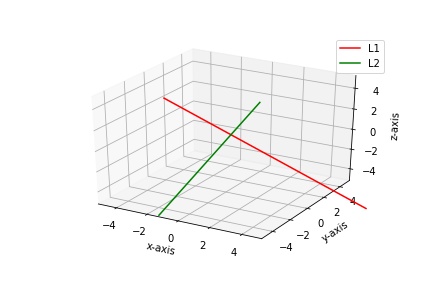
\includegraphics[width=\columnwidth]{lines.png}
	\caption{} \label{linefig1}
\end{figure}
\end{document}

%
\begin{align}
\myvec{2 & 3}\vec{x} &= k
\end{align}
%
%
\item Draw the graphs of the following equations
\begin{enumerate}[itemsep=2pt]
%\begin{multicols}{2}
\item $\myvec{1 & 1}\vec{x} = 4$
\item $\myvec{ 1 & -1}\vec{x}  = 2 $
\item $\myvec{ 3 & -1}\vec{x}  = 0$
\item $\myvec{ 2 & 1}\vec{x}  = 3$
\item $\myvec{ 1 & -1}\vec{x}  = 0$
\item $\myvec{ 1& 1}\vec{x}  = 0$
\item $\myvec{ 2& -1}\vec{x}  = 0$
\item $\myvec{ 7& -3}\vec{x}  = 2$
\item $\myvec{ 1& 1}\vec{x}  = 0$
\item $\myvec{ 1& -1}\vec{x}  = -2$
\item $\myvec{ 1& 1}\vec{x}  = 2$
\item $\myvec{ 1& 2}\vec{x}  = 6$
%\end{multicols}
\end{enumerate}
%
\solution
\begin{enumerate}
\item 
\begin{table}[!ht]
\centering
\resizebox{\columnwidth}{!}{\begin{tabular}{|c|c|c|c|} 
\hline
kind of  cake & No.of cakes & Flour& Fat\\
\hline
1st & x & 200g  &  25g \\ 
\hline
2nd& y& 100g&  50g  \\ 
\hline
Total& x+y& 5 kg=5000g&1kg=1000g \\ 
\hline
\end{tabular}}
\caption{Ingredients used in making the cake is flour and fat }
\label{opt/13/tab:table1}
\end{table}
Let the  1st kind  be $x$ and the 2nd kind be $y$  such that 
\begin{align}
x \geq 0 \\
y \geq 0 
\end{align}
According to the question,
\begin{align}
2{x} + {y} \leq 50
\\
{x} + 2{y} \leq 40
\end{align}
$\therefore$ Our problem is
\begin{align}
\max_{\vec{x}} Z &= \myvec{1& 1}\vec{x}\\
s.t. \quad \myvec{2 & 1 \\ 1& 2}\vec{x} &\preceq \myvec{50\\40} 
\end{align}
Lagrangian function is given by
\begin{equation}
\begin{aligned}
&L(\vec{x},\boldsymbol{\lambda}) \\ &= \myvec{1 & 1}\vec{x}+\lcbrak{\sbrak{\myvec{2 & 1}\vec{x}-50}} \\ &+ \sbrak{\myvec{1 & 2}\vec{x}-40}\\ &+ \sbrak{\myvec{-1 & 0}\vec{x}} +\rcbrak{\sbrak{\myvec{0 & -1}\vec{x}}}\boldsymbol{\lambda}
\end{aligned}
\end{equation}
where,
\begin{align}
\boldsymbol{\lambda} &= \myvec{\lambda_1 \\ \lambda_2 \\ \lambda_3 \\ \lambda_4 \\ \lambda_5 \\ \lambda_6}
\end{align}
Now,
\begin{align}
\nabla L(\vec{x},\boldsymbol{\lambda}) &= \myvec{1+ \myvec{2 & 1 & -1 & 0 }\boldsymbol{\lambda}\\ 1+\myvec{1 & 2 & 0 & -1}\boldsymbol{\lambda} \\ \myvec{2 & 1}\vec{x}-50\\ \myvec{1& 2}\vec{x}-40 \\  \myvec{-1 & 0}\vec{x} \\ \myvec{0 & -1}\vec{x}}
\end{align}
$\therefore$ Lagrangian matrix is given by
\begin{align}
\myvec{0 & 0 & 2 & 1& -1 & 0 \\ 0 & 0 & 1 & 2  & 0 & -1 \\ 2 & 1 & 0 & 0 & 0 & 0 \\ 1 & 2 & 0 & 0 & 0 & 0  \\ -1 & 0 & 0 & 0 & 0 & 0  \\ 0 & -1 & 0 & 0 & 0 & 0 }\myvec{\vec{x} \\ \boldsymbol{\lambda} } &= \myvec{-1 \\ -1 \\ 50\\ 4 0\\ 0 \\0 }
\end{align}
Considering $\lambda_1,\lambda_2$ as only active multiplier,
\begin{align}
\myvec{0 & 0 & 2 & 1 \\ 0 & 0 & 1 & 2 \\ 2 & 1 & 0 & 0 \\ 1 & 2 & 0 & 0}\myvec{\vec{x}\\ \boldsymbol{\lambda}} &= \myvec{-1 \\ -1 \\ 5 0\\ 40}
\end{align}
resulting in,
\begin{align}
\myvec{\vec{x} \\ \boldsymbol{\lambda}} &= \myvec{0 & 0 & 2 & 1 \\ 0 & 0 & 1 & 2 \\ 2 & 1 & 0 & 0 \\ 1& 2 & 0 & 0}^{-1}\myvec{-1 \\ -1 \\ 50 \\ 40}
\\
\implies   \myvec{\vec{x} \\ \boldsymbol{\lambda}} &= \myvec{0 & 0 & \frac{2}{3} & \frac{-1}{3} \\ 0 & 0 & \frac{-1}{3} & \frac{2}{3} \\ \frac{2}{3} & \frac{-1}{3} & 0 & 0 \\ \frac{-1}{3} & \frac{2}{3} & 0 & 0}\myvec{-1 \\ -1 \\ 50 \\ 40}
\\
\implies \myvec{\vec{x} \\ \boldsymbol{\lambda}} &= \myvec{20 \\ 10 \\ -0.3 \\ -0.3 }
\end{align}
$\because \boldsymbol{\lambda}=\myvec{-0.3 \\ -0.3} \succ \vec{0} $
\\
$\therefore$ Optimal solution is given by
\begin{align}
    \vec{x} &= \myvec{20\\10} \\
    Z &= \myvec{1& 1}\vec{x} \\
    &= \myvec{1 & 1}\myvec{20 \\ 10} \\
    &= 60
\end{align}
By using cvxpy in python ,
\begin{align}
    \vec{x}=\myvec{20\\10}\\
    Z = 60
\end{align}
Hence No.of cakes \boxed{x=20} 1st kind and  .of cakes \boxed{y=10} 2nd kind should be used to maximum No. of cakes \boxed{Z=60}.  This is
verified in Fig. \ref{opt/13/fig: Graphical Solution}.	
%
\begin{figure}[!ht]
\centering
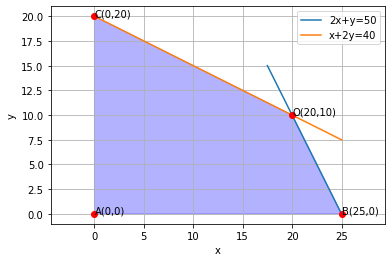
\includegraphics[width=\columnwidth]{solutions/su2021/2/13/Figure9.png}
\caption{Graphical Solution}
\label{opt/13/fig: Graphical Solution}	
\end{figure}

%\item 
\begin{table}[!ht]
\centering
\resizebox{\columnwidth}{!}{\begin{tabular}{|c|c|c|c|} 
\hline
kind of  cake & No.of cakes & Flour& Fat\\
\hline
1st & x & 200g  &  25g \\ 
\hline
2nd& y& 100g&  50g  \\ 
\hline
Total& x+y& 5 kg=5000g&1kg=1000g \\ 
\hline
\end{tabular}}
\caption{Ingredients used in making the cake is flour and fat }
\label{opt/13/tab:table1}
\end{table}
Let the  1st kind  be $x$ and the 2nd kind be $y$  such that 
\begin{align}
x \geq 0 \\
y \geq 0 
\end{align}
According to the question,
\begin{align}
2{x} + {y} \leq 50
\\
{x} + 2{y} \leq 40
\end{align}
$\therefore$ Our problem is
\begin{align}
\max_{\vec{x}} Z &= \myvec{1& 1}\vec{x}\\
s.t. \quad \myvec{2 & 1 \\ 1& 2}\vec{x} &\preceq \myvec{50\\40} 
\end{align}
Lagrangian function is given by
\begin{equation}
\begin{aligned}
&L(\vec{x},\boldsymbol{\lambda}) \\ &= \myvec{1 & 1}\vec{x}+\lcbrak{\sbrak{\myvec{2 & 1}\vec{x}-50}} \\ &+ \sbrak{\myvec{1 & 2}\vec{x}-40}\\ &+ \sbrak{\myvec{-1 & 0}\vec{x}} +\rcbrak{\sbrak{\myvec{0 & -1}\vec{x}}}\boldsymbol{\lambda}
\end{aligned}
\end{equation}
where,
\begin{align}
\boldsymbol{\lambda} &= \myvec{\lambda_1 \\ \lambda_2 \\ \lambda_3 \\ \lambda_4 \\ \lambda_5 \\ \lambda_6}
\end{align}
Now,
\begin{align}
\nabla L(\vec{x},\boldsymbol{\lambda}) &= \myvec{1+ \myvec{2 & 1 & -1 & 0 }\boldsymbol{\lambda}\\ 1+\myvec{1 & 2 & 0 & -1}\boldsymbol{\lambda} \\ \myvec{2 & 1}\vec{x}-50\\ \myvec{1& 2}\vec{x}-40 \\  \myvec{-1 & 0}\vec{x} \\ \myvec{0 & -1}\vec{x}}
\end{align}
$\therefore$ Lagrangian matrix is given by
\begin{align}
\myvec{0 & 0 & 2 & 1& -1 & 0 \\ 0 & 0 & 1 & 2  & 0 & -1 \\ 2 & 1 & 0 & 0 & 0 & 0 \\ 1 & 2 & 0 & 0 & 0 & 0  \\ -1 & 0 & 0 & 0 & 0 & 0  \\ 0 & -1 & 0 & 0 & 0 & 0 }\myvec{\vec{x} \\ \boldsymbol{\lambda} } &= \myvec{-1 \\ -1 \\ 50\\ 4 0\\ 0 \\0 }
\end{align}
Considering $\lambda_1,\lambda_2$ as only active multiplier,
\begin{align}
\myvec{0 & 0 & 2 & 1 \\ 0 & 0 & 1 & 2 \\ 2 & 1 & 0 & 0 \\ 1 & 2 & 0 & 0}\myvec{\vec{x}\\ \boldsymbol{\lambda}} &= \myvec{-1 \\ -1 \\ 5 0\\ 40}
\end{align}
resulting in,
\begin{align}
\myvec{\vec{x} \\ \boldsymbol{\lambda}} &= \myvec{0 & 0 & 2 & 1 \\ 0 & 0 & 1 & 2 \\ 2 & 1 & 0 & 0 \\ 1& 2 & 0 & 0}^{-1}\myvec{-1 \\ -1 \\ 50 \\ 40}
\\
\implies   \myvec{\vec{x} \\ \boldsymbol{\lambda}} &= \myvec{0 & 0 & \frac{2}{3} & \frac{-1}{3} \\ 0 & 0 & \frac{-1}{3} & \frac{2}{3} \\ \frac{2}{3} & \frac{-1}{3} & 0 & 0 \\ \frac{-1}{3} & \frac{2}{3} & 0 & 0}\myvec{-1 \\ -1 \\ 50 \\ 40}
\\
\implies \myvec{\vec{x} \\ \boldsymbol{\lambda}} &= \myvec{20 \\ 10 \\ -0.3 \\ -0.3 }
\end{align}
$\because \boldsymbol{\lambda}=\myvec{-0.3 \\ -0.3} \succ \vec{0} $
\\
$\therefore$ Optimal solution is given by
\begin{align}
    \vec{x} &= \myvec{20\\10} \\
    Z &= \myvec{1& 1}\vec{x} \\
    &= \myvec{1 & 1}\myvec{20 \\ 10} \\
    &= 60
\end{align}
By using cvxpy in python ,
\begin{align}
    \vec{x}=\myvec{20\\10}\\
    Z = 60
\end{align}
Hence No.of cakes \boxed{x=20} 1st kind and  .of cakes \boxed{y=10} 2nd kind should be used to maximum No. of cakes \boxed{Z=60}.  This is
verified in Fig. \ref{opt/13/fig: Graphical Solution}.	
%
\begin{figure}[!ht]
\centering
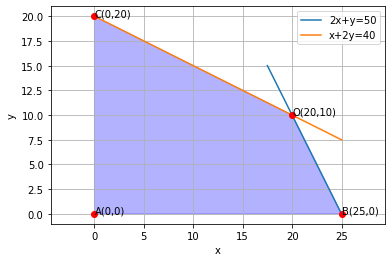
\includegraphics[width=\columnwidth]{solutions/su2021/2/13/Figure9.png}
\caption{Graphical Solution}
\label{opt/13/fig: Graphical Solution}	
\end{figure}

\end{enumerate}
\item Give the equations of two lines passing through \myvec{2 \\ 14}. How many more such lines are there, and why?
\item Find out whether the following pair of linear
equations are consistent, or inconsistent.
%
\begin{enumerate}[itemsep=2pt]
%\begin{multicols}{2}
\item
\begin{align}
\begin{split}
\myvec{3 & 2 }\vec{x}&=5
\\
\myvec{2 & -3 }\vec{x}&=7
\end{split}
\end{align}
\item
\begin{align}
\begin{split}
\myvec{2 & -3 }\vec{x}&=8
\\
\myvec{4 & -6 }\vec{x}&=9
\end{split}
\end{align}
\item
\begin{align}
\begin{split}
\myvec{\frac{3}{2} & \frac{5}{3} }\vec{x}&=7
\\
\myvec{9 & -10 }\vec{x}&=14
\end{split}
\end{align}
\item
\begin{align}
\begin{split}
\myvec{5 & -3 }\vec{x}&=11
\\
\myvec{-10 & 6 }\vec{x}&=-22
\end{split}
\end{align}
\item
\begin{align}
\begin{split}
\myvec{\frac{4}{3} & 2 }\vec{x}&=8
\\
\myvec{2 & 3 }\vec{x}&=12
\end{split}
\end{align}
%\end{multicols}
\end{enumerate}
%
\solution
\begin{enumerate}
\item The given problem can be expressed in general
as matrix inequality as:
%
\begin{align}
    \max_{\{x\}}\vec{c}^T\Vec{x}\\
    s.t \quad \Vec{A}\vec{x}\leq \vec{b} \\
    \Vec{x} \geq 0\\
    \Vec{y} \geq 0
\end{align}
where,
\begin{align}
    \Vec{c}=\myvec{1\\1}\\
    \Vec{A}=\myvec{1 & -1\\-1 & 1}\\
    \Vec{b}=\myvec{-1\\0}
\end{align}
Solving for Z by this reduction method we get
\begin{align}
    Max Z = None
\end{align}
There is no optimal maximum solution for this.
%
See Fig. \ref{sep/2/11/fig}.
\begin{figure}[h]
\centering
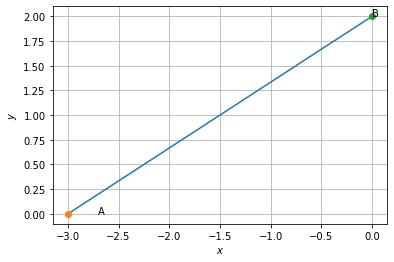
\includegraphics[width=\columnwidth]{solutions/sep/2/11/Figures/Figure.png}
\caption{Plot from python code }
\label{sep/2/11/fig}
\end{figure}

\item \input{}

\end{enumerate}
%
\item Find the slope of the line, which makes an angle of $30\degree$ of y-axis measured anticlockwise.
\item Write the equations for the x and y axes.
\item Find the equation of the line satisfying the following conditions 
\begin{enumerate}
\item passing through  the point \myvec{-4\\3} with slope $\frac{1}{2}$.
\item passing through the point \myvec{0\\0} with slope $m$.
\item passing through the point $\myvec{2\\2\sqrt{3}}$ and inclined with the x-axis at an angle of 75$\degree$.
\item Intersecting the x-axis at a distance of 3 units to the let of the origin with slope -2.
\item intersecting the y-axis at a distance of 2 units above the origin and making an angle of $30\degree$ with the positive direction of the x-axis.
\item passing through the points \myvec{-1\\1} and \myvec{2\\-4}.
\item perpendicular distance from the origin is 5 and the angle made by the perpendicular with the positive x-axis is 30$\degree$.
\end{enumerate}
%
\solution
\begin{enumerate}
\item 
\begin{align}
    \myvec{2&3&4\\
           3&4&5\\
           4&5&6}\myvec{1&-3&5\\
                        0&2&4\\
                        3&0&5}
    &=\myvec{2+0+12&-6+6+0&10+12+20\\
           3+0+15&-9+8+0&15+16+25\\
           4+0+18&-12+10+0&20+20+30}\\
    &=\myvec{14&0&42\\
             18&-1&56\\
             22&-2&70}
\end{align}

\item 
\begin{table}[!ht]
\centering
\resizebox{\columnwidth}{!}{\begin{tabular}{|c|c|c|c|} 
\hline
kind of  cake & No.of cakes & Flour& Fat\\
\hline
1st & x & 200g  &  25g \\ 
\hline
2nd& y& 100g&  50g  \\ 
\hline
Total& x+y& 5 kg=5000g&1kg=1000g \\ 
\hline
\end{tabular}}
\caption{Ingredients used in making the cake is flour and fat }
\label{opt/13/tab:table1}
\end{table}
Let the  1st kind  be $x$ and the 2nd kind be $y$  such that 
\begin{align}
x \geq 0 \\
y \geq 0 
\end{align}
According to the question,
\begin{align}
2{x} + {y} \leq 50
\\
{x} + 2{y} \leq 40
\end{align}
$\therefore$ Our problem is
\begin{align}
\max_{\vec{x}} Z &= \myvec{1& 1}\vec{x}\\
s.t. \quad \myvec{2 & 1 \\ 1& 2}\vec{x} &\preceq \myvec{50\\40} 
\end{align}
Lagrangian function is given by
\begin{equation}
\begin{aligned}
&L(\vec{x},\boldsymbol{\lambda}) \\ &= \myvec{1 & 1}\vec{x}+\lcbrak{\sbrak{\myvec{2 & 1}\vec{x}-50}} \\ &+ \sbrak{\myvec{1 & 2}\vec{x}-40}\\ &+ \sbrak{\myvec{-1 & 0}\vec{x}} +\rcbrak{\sbrak{\myvec{0 & -1}\vec{x}}}\boldsymbol{\lambda}
\end{aligned}
\end{equation}
where,
\begin{align}
\boldsymbol{\lambda} &= \myvec{\lambda_1 \\ \lambda_2 \\ \lambda_3 \\ \lambda_4 \\ \lambda_5 \\ \lambda_6}
\end{align}
Now,
\begin{align}
\nabla L(\vec{x},\boldsymbol{\lambda}) &= \myvec{1+ \myvec{2 & 1 & -1 & 0 }\boldsymbol{\lambda}\\ 1+\myvec{1 & 2 & 0 & -1}\boldsymbol{\lambda} \\ \myvec{2 & 1}\vec{x}-50\\ \myvec{1& 2}\vec{x}-40 \\  \myvec{-1 & 0}\vec{x} \\ \myvec{0 & -1}\vec{x}}
\end{align}
$\therefore$ Lagrangian matrix is given by
\begin{align}
\myvec{0 & 0 & 2 & 1& -1 & 0 \\ 0 & 0 & 1 & 2  & 0 & -1 \\ 2 & 1 & 0 & 0 & 0 & 0 \\ 1 & 2 & 0 & 0 & 0 & 0  \\ -1 & 0 & 0 & 0 & 0 & 0  \\ 0 & -1 & 0 & 0 & 0 & 0 }\myvec{\vec{x} \\ \boldsymbol{\lambda} } &= \myvec{-1 \\ -1 \\ 50\\ 4 0\\ 0 \\0 }
\end{align}
Considering $\lambda_1,\lambda_2$ as only active multiplier,
\begin{align}
\myvec{0 & 0 & 2 & 1 \\ 0 & 0 & 1 & 2 \\ 2 & 1 & 0 & 0 \\ 1 & 2 & 0 & 0}\myvec{\vec{x}\\ \boldsymbol{\lambda}} &= \myvec{-1 \\ -1 \\ 5 0\\ 40}
\end{align}
resulting in,
\begin{align}
\myvec{\vec{x} \\ \boldsymbol{\lambda}} &= \myvec{0 & 0 & 2 & 1 \\ 0 & 0 & 1 & 2 \\ 2 & 1 & 0 & 0 \\ 1& 2 & 0 & 0}^{-1}\myvec{-1 \\ -1 \\ 50 \\ 40}
\\
\implies   \myvec{\vec{x} \\ \boldsymbol{\lambda}} &= \myvec{0 & 0 & \frac{2}{3} & \frac{-1}{3} \\ 0 & 0 & \frac{-1}{3} & \frac{2}{3} \\ \frac{2}{3} & \frac{-1}{3} & 0 & 0 \\ \frac{-1}{3} & \frac{2}{3} & 0 & 0}\myvec{-1 \\ -1 \\ 50 \\ 40}
\\
\implies \myvec{\vec{x} \\ \boldsymbol{\lambda}} &= \myvec{20 \\ 10 \\ -0.3 \\ -0.3 }
\end{align}
$\because \boldsymbol{\lambda}=\myvec{-0.3 \\ -0.3} \succ \vec{0} $
\\
$\therefore$ Optimal solution is given by
\begin{align}
    \vec{x} &= \myvec{20\\10} \\
    Z &= \myvec{1& 1}\vec{x} \\
    &= \myvec{1 & 1}\myvec{20 \\ 10} \\
    &= 60
\end{align}
By using cvxpy in python ,
\begin{align}
    \vec{x}=\myvec{20\\10}\\
    Z = 60
\end{align}
Hence No.of cakes \boxed{x=20} 1st kind and  .of cakes \boxed{y=10} 2nd kind should be used to maximum No. of cakes \boxed{Z=60}.  This is
verified in Fig. \ref{opt/13/fig: Graphical Solution}.	
%
\begin{figure}[!ht]
\centering
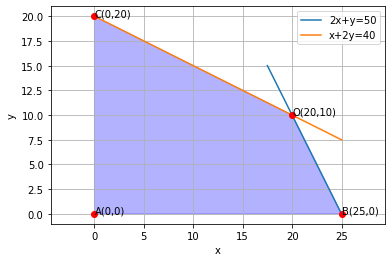
\includegraphics[width=\columnwidth]{solutions/su2021/2/13/Figure9.png}
\caption{Graphical Solution}
\label{opt/13/fig: Graphical Solution}	
\end{figure}

\end{enumerate}

\item Find the direction vectors and and y-intercepts  of the following lines 
\begin{enumerate}
\item $\myvec{1 & 7}\vec{x} = 0$.
\item $\myvec{6 & 3}\vec{x} = 5$.
\item $\myvec{0 & 1}\vec{x} = 0$.
\end{enumerate}

\item Find the perpendicular distances of the following lines from the origin and angle between the perpendicular and the positive x-axis.
\begin{enumerate}
\item $\myvec{1 & -\sqrt{3}}\vec{x} = -8$.
\item $\myvec{0 & 1}\vec{x} = 2$.
\item $\myvec{1 & -1}\vec{x} = 4$.
\end{enumerate}

\item Find the equation of the line parallel to the line 
\begin{align}
\myvec{3 & -4}\vec{x} = -2
\end{align}
%
and passing through the point \myvec{-2\\3}.
%
\item The hypotenuse of a right angled triangle has its ends at the points \myvec{1\\3} and \myvec{-4\\1}. Find an equation of the legs of the triangle.

\item If the lines
%
%
\begin{align}
\myvec{-3 & 1}\vec{x} &= 1
\\
\myvec{-1 & 2}\vec{x} &= 3
\end{align}
%
are equally inclined to the line
%
\begin{align}
\myvec{-m & 1}\vec{x} &= 4,
\end{align}
%
find the value of $m$.
%
\item The sum of the perpendicular distances of a variable point $\vec{P}$ from the lines
%
\begin{align}
\myvec{1 & 1}\vec{x} &= 0
\\
\myvec{3 & -2}\vec{x} &= -7
\end{align}
%
is always 10.  Show that $\vec{P}$ must move on a line.
%
\item Find the equation of the line which is equidistant from parallel lines
%
\begin{align}
\myvec{9 & 7}\vec{x} &= 7
\\
\myvec{3 & 2}\vec{x} &= -6.
\end{align}
%
\solution

\begin{table}[!ht]
\centering
\resizebox{\columnwidth}{!}{\begin{tabular}{|c|c|c|c|} 
\hline
kind of  cake & No.of cakes & Flour& Fat\\
\hline
1st & x & 200g  &  25g \\ 
\hline
2nd& y& 100g&  50g  \\ 
\hline
Total& x+y& 5 kg=5000g&1kg=1000g \\ 
\hline
\end{tabular}}
\caption{Ingredients used in making the cake is flour and fat }
\label{opt/13/tab:table1}
\end{table}
Let the  1st kind  be $x$ and the 2nd kind be $y$  such that 
\begin{align}
x \geq 0 \\
y \geq 0 
\end{align}
According to the question,
\begin{align}
2{x} + {y} \leq 50
\\
{x} + 2{y} \leq 40
\end{align}
$\therefore$ Our problem is
\begin{align}
\max_{\vec{x}} Z &= \myvec{1& 1}\vec{x}\\
s.t. \quad \myvec{2 & 1 \\ 1& 2}\vec{x} &\preceq \myvec{50\\40} 
\end{align}
Lagrangian function is given by
\begin{equation}
\begin{aligned}
&L(\vec{x},\boldsymbol{\lambda}) \\ &= \myvec{1 & 1}\vec{x}+\lcbrak{\sbrak{\myvec{2 & 1}\vec{x}-50}} \\ &+ \sbrak{\myvec{1 & 2}\vec{x}-40}\\ &+ \sbrak{\myvec{-1 & 0}\vec{x}} +\rcbrak{\sbrak{\myvec{0 & -1}\vec{x}}}\boldsymbol{\lambda}
\end{aligned}
\end{equation}
where,
\begin{align}
\boldsymbol{\lambda} &= \myvec{\lambda_1 \\ \lambda_2 \\ \lambda_3 \\ \lambda_4 \\ \lambda_5 \\ \lambda_6}
\end{align}
Now,
\begin{align}
\nabla L(\vec{x},\boldsymbol{\lambda}) &= \myvec{1+ \myvec{2 & 1 & -1 & 0 }\boldsymbol{\lambda}\\ 1+\myvec{1 & 2 & 0 & -1}\boldsymbol{\lambda} \\ \myvec{2 & 1}\vec{x}-50\\ \myvec{1& 2}\vec{x}-40 \\  \myvec{-1 & 0}\vec{x} \\ \myvec{0 & -1}\vec{x}}
\end{align}
$\therefore$ Lagrangian matrix is given by
\begin{align}
\myvec{0 & 0 & 2 & 1& -1 & 0 \\ 0 & 0 & 1 & 2  & 0 & -1 \\ 2 & 1 & 0 & 0 & 0 & 0 \\ 1 & 2 & 0 & 0 & 0 & 0  \\ -1 & 0 & 0 & 0 & 0 & 0  \\ 0 & -1 & 0 & 0 & 0 & 0 }\myvec{\vec{x} \\ \boldsymbol{\lambda} } &= \myvec{-1 \\ -1 \\ 50\\ 4 0\\ 0 \\0 }
\end{align}
Considering $\lambda_1,\lambda_2$ as only active multiplier,
\begin{align}
\myvec{0 & 0 & 2 & 1 \\ 0 & 0 & 1 & 2 \\ 2 & 1 & 0 & 0 \\ 1 & 2 & 0 & 0}\myvec{\vec{x}\\ \boldsymbol{\lambda}} &= \myvec{-1 \\ -1 \\ 5 0\\ 40}
\end{align}
resulting in,
\begin{align}
\myvec{\vec{x} \\ \boldsymbol{\lambda}} &= \myvec{0 & 0 & 2 & 1 \\ 0 & 0 & 1 & 2 \\ 2 & 1 & 0 & 0 \\ 1& 2 & 0 & 0}^{-1}\myvec{-1 \\ -1 \\ 50 \\ 40}
\\
\implies   \myvec{\vec{x} \\ \boldsymbol{\lambda}} &= \myvec{0 & 0 & \frac{2}{3} & \frac{-1}{3} \\ 0 & 0 & \frac{-1}{3} & \frac{2}{3} \\ \frac{2}{3} & \frac{-1}{3} & 0 & 0 \\ \frac{-1}{3} & \frac{2}{3} & 0 & 0}\myvec{-1 \\ -1 \\ 50 \\ 40}
\\
\implies \myvec{\vec{x} \\ \boldsymbol{\lambda}} &= \myvec{20 \\ 10 \\ -0.3 \\ -0.3 }
\end{align}
$\because \boldsymbol{\lambda}=\myvec{-0.3 \\ -0.3} \succ \vec{0} $
\\
$\therefore$ Optimal solution is given by
\begin{align}
    \vec{x} &= \myvec{20\\10} \\
    Z &= \myvec{1& 1}\vec{x} \\
    &= \myvec{1 & 1}\myvec{20 \\ 10} \\
    &= 60
\end{align}
By using cvxpy in python ,
\begin{align}
    \vec{x}=\myvec{20\\10}\\
    Z = 60
\end{align}
Hence No.of cakes \boxed{x=20} 1st kind and  .of cakes \boxed{y=10} 2nd kind should be used to maximum No. of cakes \boxed{Z=60}.  This is
verified in Fig. \ref{opt/13/fig: Graphical Solution}.	
%
\begin{figure}[!ht]
\centering
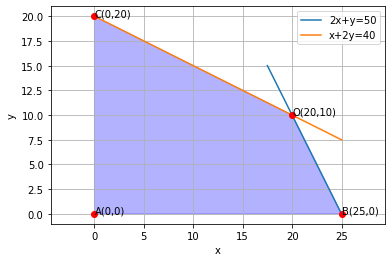
\includegraphics[width=\columnwidth]{solutions/su2021/2/13/Figure9.png}
\caption{Graphical Solution}
\label{opt/13/fig: Graphical Solution}	
\end{figure}

\item Determine the ratio in which the line 
\begin{align}
\myvec{2 & 1}\vec{x} - 4 = 0
\end{align}
%
divides the line segment joining the points $\vec{A}=\myvec{2\\-2}, \vec{B}=\myvec{3\\7}$.
\item A line perpendicular to the line segment joining the points \myvec{1\\0} and \myvec{2\\3} divides it in the ratio $1:n$.  Find the equation of the line.
\\
\solution

Let $\vec{p} = \myvec{1\\2\\3}$ be a point on the line L.
Direction vector of the  line perpendicular to the given plane is
\begin{align}
 \myvec{1\\2\\-5}
\end{align}
Thus, the equation of required line is
\begin{align}
    L: \quad \vec{x}&=\vec{p}+\lambda\vec{a}\\ &=\myvec{1\\2\\3}+\lambda\myvec{1\\2\\-5}
\end{align}
See Fig.  \ref{aug/2/34/plot}.
\begin{figure}[!h]
 \centering
 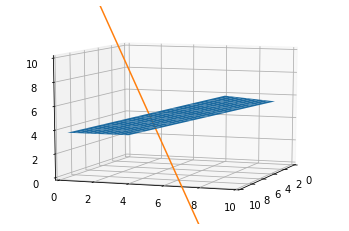
\includegraphics[width=\columnwidth]{solutions/aug/2/34/figs/Assignment4.png}
 \caption{Plot of plane and the line}
 \label{aug/2/34/plot}
\end{figure}




\item Find the equation of a line that cuts off equal intercepts on the coordinate axes and passes through the point \myvec{2\\3}.
\\
\solution
Let the equation of line be
\begin{align}
    \vec{n}^\top\brak{\vec{x}-\vec{P}}=0
\end{align}
So the perpendicular from the origin meets the line at $\vec{P}= \myvec{-2 \\ 9}$.Since,
\begin{align}
   \vec{n}&= \vec{P}-\vec{O}\\
   &=\myvec{-2-0\\9-0}\\
   &=\myvec{-2\\9}
\end{align}
is the normal vector where $\vec{O}$ is the origin then 
is the direction vector, Hence the equation of line is given by
\begin{align}
   \myvec{-2 & 9}\brak{\vec{x}-\myvec{-2 \\ 9}}&=0 \\
\implies     \myvec{-2 & 9}\vec{x}&= 85
\end{align}
    See Fig. \ref{aug/2/21/fig:my_label}
\begin{figure}[htp]
    \centering
    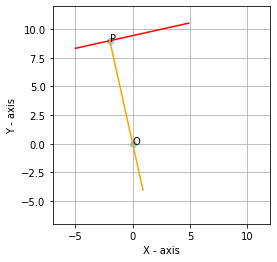
\includegraphics{solutions/aug/2/21/Assignment_4.png}
    \caption{graph}
    \label{aug/2/21/fig:my_label}
\end{figure}


\item Find the equation of the line passing through the point \myvec{2\\2} and cutting off intercepts on the axes whose sum is 9.
\item Find the equation of the line through the point \myvec{0\\2} making an angle $\frac{2\pi}{3}$ with the positive x-axis.  Also, find the equation of the line parallel to it and crossing the y-axis at a distance of 2 units below the origin.
\\
\solution

Let $\vec{p} = \myvec{1\\2\\3}$ be a point on the line L.
Direction vector of the  line perpendicular to the given plane is
\begin{align}
 \myvec{1\\2\\-5}
\end{align}
Thus, the equation of required line is
\begin{align}
    L: \quad \vec{x}&=\vec{p}+\lambda\vec{a}\\ &=\myvec{1\\2\\3}+\lambda\myvec{1\\2\\-5}
\end{align}
See Fig.  \ref{aug/2/34/plot}.
\begin{figure}[!h]
 \centering
 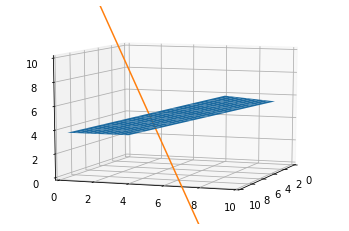
\includegraphics[width=\columnwidth]{solutions/aug/2/34/figs/Assignment4.png}
 \caption{Plot of plane and the line}
 \label{aug/2/34/plot}
\end{figure}



%
\item The perpendicular from the origin to a line meets it at a point \myvec{-2\\9}, find the equation of the line.
\\
\solution
Let the equation of line be
\begin{align}
    \vec{n}^\top\brak{\vec{x}-\vec{P}}=0
\end{align}
So the perpendicular from the origin meets the line at $\vec{P}= \myvec{-2 \\ 9}$.Since,
\begin{align}
   \vec{n}&= \vec{P}-\vec{O}\\
   &=\myvec{-2-0\\9-0}\\
   &=\myvec{-2\\9}
\end{align}
is the normal vector where $\vec{O}$ is the origin then 
is the direction vector, Hence the equation of line is given by
\begin{align}
   \myvec{-2 & 9}\brak{\vec{x}-\myvec{-2 \\ 9}}&=0 \\
\implies     \myvec{-2 & 9}\vec{x}&= 85
\end{align}
    See Fig. \ref{aug/2/21/fig:my_label}
\begin{figure}[htp]
    \centering
    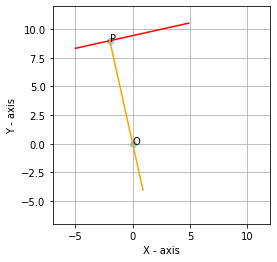
\includegraphics{solutions/aug/2/21/Assignment_4.png}
    \caption{graph}
    \label{aug/2/21/fig:my_label}
\end{figure}



%\end{enumerate}
%
\item Find the shortest distance between the lines 
\begin{align}
\frac{x+1}{7} = \frac{y+1}{-6} &= \frac{z+1}{1}, 
\\
\frac{x-3}{1} = \frac{y-5}{-2} &= \frac{z-7}{1} 
\end{align}
%
\solution 
\begin{enumerate}
\item 
Let $\vec{p} = \myvec{1\\2\\3}$ be a point on the line L.
Direction vector of the  line perpendicular to the given plane is
\begin{align}
 \myvec{1\\2\\-5}
\end{align}
Thus, the equation of required line is
\begin{align}
    L: \quad \vec{x}&=\vec{p}+\lambda\vec{a}\\ &=\myvec{1\\2\\3}+\lambda\myvec{1\\2\\-5}
\end{align}
See Fig.  \ref{aug/2/34/plot}.
\begin{figure}[!h]
 \centering
 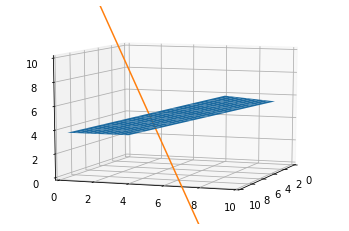
\includegraphics[width=\columnwidth]{solutions/aug/2/34/figs/Assignment4.png}
 \caption{Plot of plane and the line}
 \label{aug/2/34/plot}
\end{figure}



\end{enumerate}
\item Find the shortest distance between the lines 
\begin{align}
L_1: \quad \vec{x} &= \myvec{1\\2\\3} + \lambda_1\myvec{1 \\ -3 \\2}
\\
L_2: \quad \vec{x} &= \myvec{4\\5\\6} + \lambda_2\myvec{2 \\ 3 \\1}
\end{align}
%
\solution 
We have,
\begin{align}
    \label{sep/2/23/eq:3}                       
    L_{1}: \: \Vec{x}={}&\Vec{a_{1}}+\lambda_{1}\Vec{b_{1}}\\
    \label{sep/2/23/eq:4}
    L_{2}: \: \Vec{x}={}&\Vec{a_{2}}+\lambda_{2}\Vec{b_{2}}
\end{align}
where $\Vec{a_{i}},\Vec{b_{i}}$ are positional vector, slope vector of line $L_{i}$ respectively.\\
\begin{align}
\Vec{b_{1}}\neq k \Vec{b_{2}},
\end{align}
the lines are not parallel to each other.
If $L_{1}$ and $L_{2}$ intersect at a point,
\begin{align}
    \label{sep/2/23/eq:5}
    \myvec{1 \\ 2\\ 3 } +\lambda_{1}\myvec{1 \\ -3 \\ 2} = \myvec{4 \\ 5\\ 6} + \lambda_{2}\myvec{2 \\ 3 \\ 1} \\
    \label{sep/2/23/eq:6}
\implies 
    \myvec{1 & -2\\ -3 &-3 \\ 2 & -1}\myvec{\lambda_{1}\\ \lambda_{2}}=
    \myvec{3 \\ 3\\ 3 }
\end{align}
Rown reducing the augmented matrix,
\begin{multline}
    \myvec{1 & -2 & 3\\ -3 &-3 & 3\\ 2 & -1 & 3} \xleftrightarrow{R_{2}\leftarrow R_{2}+3R_{1}}
     \myvec{1 & -2 & 3\\ 0 &3 & 9\\ 2 & -1 & 3}\\
     \xleftrightarrow{R_{3}\leftarrow R_{3}-2R_{1}}
     \myvec{1 & -2 & 3\\ 0 &3 & 9\\ 0 & 3 & -3}
   \xleftrightarrow[R_{3}\leftarrow R_{3}-3R_{2}]{R_{2}\leftarrow\frac{R_{2}}{3}}
    \myvec{1 & -2 & 3\\ 0 & 1 & 9\\ 0 & 0 & -3}
\end{multline}
$\therefore$ the rank of the matrix = 3. Hence the lines do not intersect and 
$L_{1}$ and $L_{2}$ are skew lines.  Let $d$ be the shortest distance and $\Vec{p_{1}}, \Vec{p_{2}}$ be positional vectors of its end points.  Then, 
%For $d$ to be shortest, we know that,
\begin{align}
    \label{sep/2/23/eq:9}
    \Vec{b_{1}}^\top\brak{\Vec{p_{2}}-\Vec{p_{1}}}=0\\
    \label{sep/2/23/eq:10}
     \Vec{b_{2}}^\top\brak{\Vec{p_{2}}-\Vec{p_{1}}}=0\\
     \label{sep/2/23/eq:11}
     \Vec{b_{1}}^\top\brak{\brak{\Vec{a}_{2} - \Vec{a}_{1}}}+\myvec{\Vec{b_{2}} & \Vec{b}_{1}}\myvec{\lambda_{1} \\ \lambda_{2}}=0\\
     \label{sep/2/23/eq:12}
     \Vec{b_{2}}^\top\brak{\brak{\Vec{a}_{2} - \Vec{a}_{1}}}+\myvec{\Vec{b_{2}} & \Vec{b_{1}}}\myvec{\lambda_{1} \\ \lambda_{2}}=0
\end{align}
Let 
\begin{align}
\label{sep/2/23/eq:13}
    \Vec{B}&=\myvec{\Vec{b_{2}} & \Vec{b}_{1}} & \Vec{B}^\top&=\myvec{\Vec{b_{2}}^\top \\ \Vec{b_{1}}^\top}
\end{align}
By combining equations \eqref{sep/2/23/eq:11} and \eqref{sep/2/23/eq:12} and writing in terms of $\Vec{B}$ and $\Vec{B}^\top$ using \eqref{sep/2/23/eq:13}, we get
\begin{align}
    \label{sep/2/23/eq:14}
    \Vec{B}^\top\Vec{B}\myvec{\lambda_{2} \\ -\lambda_{1}}= \Vec{B}^\top\brak{\Vec{a}_{1} - \Vec{a}_{2}}
\end{align}
By putting the values of $a_{1},a_{2},b_{1},b_{2}$ in \eqref{sep/2/23/eq:14}, we get
\begin{align}
    \label{sep/2/23/eq:15}
    \myvec{14 & -5 \\ -5 & 14}\myvec{\lambda_{2} \\ -\lambda_{1}}=\myvec{-18 \\ 0}
\end{align}
Solving \eqref{sep/2/23/eq:15}, we get
\begin{align}
    \label{sep/2/23/eq:16}
    \myvec{\lambda_{2} \\ -\lambda_{1}}=\myvec{-1.4736 \\ -0.5263}
\end{align}
Substituting the value of $\lambda_{1}$ and $\lambda_{2}$ in \eqref{sep/2/23/eq:3} and \eqref{sep/2/23/eq:4}, we get
\begin{align}
    \label{sep/2/23/eq:17}
    \Vec{p_{1}} &= \myvec{1.5263\\ 0.4210 \\ 4.0526 }   &    \Vec{p_{2}}&=\myvec{ 1.0526\\0.5789\\4.5263}
\end{align}
Hence, the shortest distance between these two skew lines is
\begin{align}
    \label{sep/2/23/eq:18}
   d= \norm{\Vec{p_{2}}-\Vec{p_{1}}} = 0.6882
\end{align}
\begin{figure}[h]
\centering
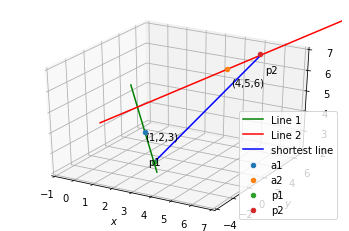
\includegraphics[width=\columnwidth]{solutions/sep/2/23/Figures/q4.png}
\caption{Plot of skew lines}
\end{figure}


\item Find the equation of the planes that passes through three points
\begin{enumerate}
\item \myvec{1\\1\\-1}, \myvec{6\\4\\-5}, \myvec{-4\\-2\\3}
\item \myvec{1\\1\\0}, \myvec{1\\2\\1}, \myvec{-2\\2\\-1}.
\end{enumerate}
\solution
\begin{enumerate}
    \item 

If the equation of the plane is given by
\begin{align}
\vec{n}^T\vec{x} = 1,
\end{align}
\begin{align}
\myvec{1&1&-1 \\ 6&4&-5 \\ -4&-2&3} \vec{n} &= \myvec{1\\1\\1}
\end{align}
Row reducing the augmented matrix, 
\begin{align}
\myvec{1 & 0 & -0.5 & -1.5\\0 & 1 & -0.5 & 2.5\\0 & 0 & 0 & 0}
\end{align}
which yields the  equation of the line
\begin{align}
\vec{x} &= \myvec{1 \\ 6 \\ -4}+\lambda\myvec{0 \\ -2 \\2}
\end{align}
and is plotted in Fig. \ref{linform/38/a/Plot of the line}.
\begin{figure}[ht]
\centering
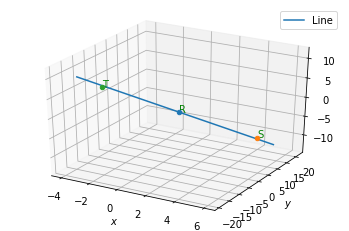
\includegraphics[width=\columnwidth]{solutions/su2021/2/36/a/download (5).png}
\caption{plot of the line}
\label{linform/38/a/Plot of the line}
\end{figure}



\end{enumerate}
\item Find the intercepts cut off by the plane 
$
\myvec{2 & 1 & 1}\vec{x}=5.
$
\item Find the equaion of the plane with intercept 3 on the y-axis and parallel to ZOX plane.
\\
\solution

\begin{table}[!ht]
\centering
\resizebox{\columnwidth}{!}{\begin{tabular}{|c|c|c|c|} 
\hline
kind of  cake & No.of cakes & Flour& Fat\\
\hline
1st & x & 200g  &  25g \\ 
\hline
2nd& y& 100g&  50g  \\ 
\hline
Total& x+y& 5 kg=5000g&1kg=1000g \\ 
\hline
\end{tabular}}
\caption{Ingredients used in making the cake is flour and fat }
\label{opt/13/tab:table1}
\end{table}
Let the  1st kind  be $x$ and the 2nd kind be $y$  such that 
\begin{align}
x \geq 0 \\
y \geq 0 
\end{align}
According to the question,
\begin{align}
2{x} + {y} \leq 50
\\
{x} + 2{y} \leq 40
\end{align}
$\therefore$ Our problem is
\begin{align}
\max_{\vec{x}} Z &= \myvec{1& 1}\vec{x}\\
s.t. \quad \myvec{2 & 1 \\ 1& 2}\vec{x} &\preceq \myvec{50\\40} 
\end{align}
Lagrangian function is given by
\begin{equation}
\begin{aligned}
&L(\vec{x},\boldsymbol{\lambda}) \\ &= \myvec{1 & 1}\vec{x}+\lcbrak{\sbrak{\myvec{2 & 1}\vec{x}-50}} \\ &+ \sbrak{\myvec{1 & 2}\vec{x}-40}\\ &+ \sbrak{\myvec{-1 & 0}\vec{x}} +\rcbrak{\sbrak{\myvec{0 & -1}\vec{x}}}\boldsymbol{\lambda}
\end{aligned}
\end{equation}
where,
\begin{align}
\boldsymbol{\lambda} &= \myvec{\lambda_1 \\ \lambda_2 \\ \lambda_3 \\ \lambda_4 \\ \lambda_5 \\ \lambda_6}
\end{align}
Now,
\begin{align}
\nabla L(\vec{x},\boldsymbol{\lambda}) &= \myvec{1+ \myvec{2 & 1 & -1 & 0 }\boldsymbol{\lambda}\\ 1+\myvec{1 & 2 & 0 & -1}\boldsymbol{\lambda} \\ \myvec{2 & 1}\vec{x}-50\\ \myvec{1& 2}\vec{x}-40 \\  \myvec{-1 & 0}\vec{x} \\ \myvec{0 & -1}\vec{x}}
\end{align}
$\therefore$ Lagrangian matrix is given by
\begin{align}
\myvec{0 & 0 & 2 & 1& -1 & 0 \\ 0 & 0 & 1 & 2  & 0 & -1 \\ 2 & 1 & 0 & 0 & 0 & 0 \\ 1 & 2 & 0 & 0 & 0 & 0  \\ -1 & 0 & 0 & 0 & 0 & 0  \\ 0 & -1 & 0 & 0 & 0 & 0 }\myvec{\vec{x} \\ \boldsymbol{\lambda} } &= \myvec{-1 \\ -1 \\ 50\\ 4 0\\ 0 \\0 }
\end{align}
Considering $\lambda_1,\lambda_2$ as only active multiplier,
\begin{align}
\myvec{0 & 0 & 2 & 1 \\ 0 & 0 & 1 & 2 \\ 2 & 1 & 0 & 0 \\ 1 & 2 & 0 & 0}\myvec{\vec{x}\\ \boldsymbol{\lambda}} &= \myvec{-1 \\ -1 \\ 5 0\\ 40}
\end{align}
resulting in,
\begin{align}
\myvec{\vec{x} \\ \boldsymbol{\lambda}} &= \myvec{0 & 0 & 2 & 1 \\ 0 & 0 & 1 & 2 \\ 2 & 1 & 0 & 0 \\ 1& 2 & 0 & 0}^{-1}\myvec{-1 \\ -1 \\ 50 \\ 40}
\\
\implies   \myvec{\vec{x} \\ \boldsymbol{\lambda}} &= \myvec{0 & 0 & \frac{2}{3} & \frac{-1}{3} \\ 0 & 0 & \frac{-1}{3} & \frac{2}{3} \\ \frac{2}{3} & \frac{-1}{3} & 0 & 0 \\ \frac{-1}{3} & \frac{2}{3} & 0 & 0}\myvec{-1 \\ -1 \\ 50 \\ 40}
\\
\implies \myvec{\vec{x} \\ \boldsymbol{\lambda}} &= \myvec{20 \\ 10 \\ -0.3 \\ -0.3 }
\end{align}
$\because \boldsymbol{\lambda}=\myvec{-0.3 \\ -0.3} \succ \vec{0} $
\\
$\therefore$ Optimal solution is given by
\begin{align}
    \vec{x} &= \myvec{20\\10} \\
    Z &= \myvec{1& 1}\vec{x} \\
    &= \myvec{1 & 1}\myvec{20 \\ 10} \\
    &= 60
\end{align}
By using cvxpy in python ,
\begin{align}
    \vec{x}=\myvec{20\\10}\\
    Z = 60
\end{align}
Hence No.of cakes \boxed{x=20} 1st kind and  .of cakes \boxed{y=10} 2nd kind should be used to maximum No. of cakes \boxed{Z=60}.  This is
verified in Fig. \ref{opt/13/fig: Graphical Solution}.	
%
\begin{figure}[!ht]
\centering
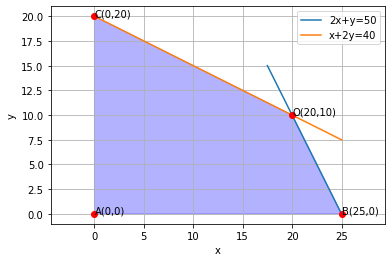
\includegraphics[width=\columnwidth]{solutions/su2021/2/13/Figure9.png}
\caption{Graphical Solution}
\label{opt/13/fig: Graphical Solution}	
\end{figure}

\item Find the equation of the plane passing through the intersection of the planes 
$
\myvec{2 & 2 & -3}\vec{x}=7
$
 and 
$
\myvec{2 & 5 & 3}\vec{x}=9
$
and the pont \myvec{2\\1\\3}.
%
\\
\solution
% The equation of a plane $P$ passing through the intersection of two planes $P_{1}$ and $P_{2}$ is given by,
% \begin{align}
%    P : P_{1} + \lambda P_{2}\label{sep/2/27/eq1}
% \end{align}
\begin{lemma}
The equation of a plane passing through the intersection of two planes and given point will be\\
% \begin{align}
% P : P_{1} + \lambda P_{2}\label{sep/2/27/eq1}
% \end{align}
Let 
\begin{align}
P_1: \quad \vec{n_{1}}^T\vec{x}&=c_{1}\\ P_2: \quad  \vec{n_{2}}^T\vec{x}&=c_{2}
\end{align}
Then, 
\begin{align}
P: \quad \vec{n^T\vec{x}}&=c
\end{align}
%Point through which Plane $P$ is passing is $A$\\
where
\begin{align}
\label{sep/2/27/lemma}
\vec{n} &= \vec{n_{1}} + \brak{\frac{c_{1} - \vec{n_{1}}^T\vec{A}}{\vec{n_{2}}^T\vec{A}- c_{2}}}\vec{n_{2}}\\
c &= c_{1} + \brak{\frac{c_{1} - \vec{A}\vec{n_{1}}^T}{\vec{A}\vec{n_{2}}^T- c_{2}}}c_{2}
\end{align}
\end{lemma}
\begin{proof}
$P$ has the equation
\begin{align}
\vec{n_{1}}^T\vec{x} + \lambda\brak{\vec{n_{2}}^T\vec{x}} = c_{1} + \lambda\brak{c_{2}}\\
\implies \brak{\vec{n_{1}}+\lambda\vec{n_{2}}}^T\vec{x} = c_{1} + \lambda\brak{c_{2}}
\end{align}
Then
\begin{align}\label{sep/2/27/eq:12}
\vec{n} &= \vec{n_{1}} + \lambda\vec{n_{2}}\\
c &= c_{1} + \lambda c_{2}
\end{align}
Given that plane $P$ passes through point $\vec{A}$ then
\begin{align}
\brak{\vec{n_{1}}+\lambda\vec{n_{2}}}^T\vec{A} &= c_{1} + \lambda\brak{c_{2}}\\
\implies \lambda &= \frac{c_{1} - \vec{n_{1}}^T\vec{A}}{\vec{n_{2}}^T\vec{A}- c_{2}}
\end{align}
Substituting $\lambda$ in \eqref{sep/2/27/eq:12} yields \ref{sep/2/27/lemma}.
% \begin{align}
% \vec{n}^T &= \vec{n_{1}}^T + \brak{\frac{c_{1} - \vec{n_{1}}^T\vec{A}}{\vec{n_{2}}^T\vec{A}- c_{2}}}\vec{n_{2}}^T\\
% c &= c_{1} + \brak{\frac{c_{1} - \vec{n_{1}}^T\vec{A}}{\vec{n_{2}}^T\vec{A}- c_{2}}}c_{2}
% \end{align}
 \end{proof}
For the given problem 
\begin{align}
\vec{n_{1}}=\myvec{2\\2\\-3}\\
\vec{n_{2}} =\myvec{2\\5\\3}\\
c_{1} = 7\\
c_{2} = 9
\end{align}
By substituting the given values,
\begin{align}
\lambda &= \frac{10}{9}\\
\vec{n} &= \myvec{\frac{38}{9}\\\frac{68}{9}\\\frac{1}{3}}\\
c &= 17
\end{align}
So the equation of plane $P$ is given by
\begin{align}
\myvec{\frac{38}{9}&\frac{68}{9}&\frac{1}{3}}\vec{x} &= 17
\end{align}
See Fig. \ref{sep/2/27/fig:Line }.	
\begin{figure}[!ht]
\centering
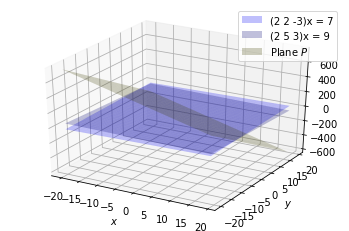
\includegraphics[ width=\columnwidth]{solutions/sep/2/27/Figure/EE3900_Assignment_4.png}
\caption{Plane $P$ passing through intersection of $P_{1}$ and $P_{2}$ and through a point $\vec{A}$}
\label{sep/2/27/fig:Line }	
\end{figure}



\item  Find the equation of the plane through the intersection of the planes
$
\myvec{1 & 1 & 1}\vec{x}=1
$
 and 
$
\myvec{2 & 3 & 4}\vec{x}=5
$
which is perpendicular to the plane 
$
\myvec{1 & -1 & 1}\vec{x}=0.
$
%
\\
\solution
% The equation of a plane $P$ passing through the line of intersection of the planes $P_{1}$ and $P_{2}$ has the form,
% \begin{align}
%    P : P_{1} + \lambda P_{2}\label{sep/2/28eq1}
% \end{align}
% %
% General equation of plane is given by
% \begin{align}
%     \vec{n}^T\vec{x}=c
% \end{align}
% Where $\vec{n}$ is normal vector to the plane
\begin{lemma}
   The equation of a plane passing through intersection of planes
   \begin{align}
    \vec{n_{1}}^T\vec{x}&=c_{1}\\ \vec{n_{2}}^T\vec{x}&=c_{2}
   \end{align}
   and perpendicular to plane
   \begin{align}
     \vec{n_{3}}^T\vec{x}&=c_{3}
   \end{align}
   is given by 
   \begin{align}
      \vec{n_{4}}^T\vec{x}&=c_{4}
   \end{align}
   where 
   \begin{align}
       \vec{n_{4}} = \vec{n_{1}} - \brak{\frac{\vec{n_{3}^T\vec{n_1}}}{\vec{n_{3}^T\vec{n_2}}}}\vec{n_2}\\
       c_{4} = c_{1} - \brak{\frac{\vec{n_{3}^T\vec{n_1}}}{\vec{n_{3}^T\vec{n_2}}}}c_{2}
   \end{align}
\end{lemma}
\begin{proof}
   Let $P$ be the plane that passes through intersection 2 given planes.\\  From \eqref{sep/2/28/eq1}, equation of $P$ has the form,
   \begin{align}
       \vec{n_{1}}^T\vec{x} + \lambda\brak{\vec{n_{2}}^T\vec{x}} = c_{1} + \lambda\brak{c_{2}}\\
       \implies \brak{\vec{n_{1}}+\lambda\vec{n_{2}}}^T\vec{x} = c_{1} + \lambda\brak{c_{2}}
   \end{align}
  Normal vector to plane $P$ is,
 \begin{align}
     \vec{n_{4}} = \vec{n_{1}}+\lambda\vec{n_{2}}
 \end{align}
 As $P$ is perpendicular to the third plane i.e. angle between normal vectors is $90\degree$, 
 \begin{align}
     &\cos\brak{90\degree} = 0 = \dfrac{\vec{n_{3}}^T\vec{n_{4}}}{\norm{\vec{n_{3}}}\norm{\vec{n_{4}}}}\\
    \implies &\vec{n_{3}}^T\vec{n_{4}} = 0\\
    \implies &\vec{n_{3}}^T\brak{\vec{n_{1}}+\lambda\vec{n_{2}}} = 0\\
    \implies &\lambda = \frac{-\vec{n_{3}^T\vec{n_1}}}{\vec{n_{3}^T\vec{n_2}}}
 \end{align}
 Therefore equation of plane $P$ is,
 \begin{align}
     \brak{\vec{n_{1}} - \brak{\frac{\vec{n_{3}^T\vec{n_1}}}{\vec{n_{3}^T\vec{n_2}}}}\vec{n_2}}^T\vec{x} = c_{1} - \brak{\frac{\vec{n_{3}^T\vec{n_1}}}{\vec{n_{3}^T\vec{n_2}}}}c_{2}
 \end{align}
\end{proof}
For the given problem,
\begin{align}
  \vec{n_{1}}=\myvec{1\\1\\1}\\c_{1}=1,
  \vec{n_{2}}=\myvec{2\\3\\4},
     c_{2}=5\\
  \vec{n_{3}}=\myvec{1\\-1\\1}\\c_{3}=0 
 \end{align}
Solving the above we get,
\begin{align}
    \lambda = \frac{-1}{3},
    \vec{n_{4}} = \myvec{\frac{1}{3}\\0\\\frac{-1}{3}},
    c_{4} = \frac{-2}{3}
\end{align}
We have equation of the plane as,
\begin{align}
    \myvec{\frac{1}{3}&0&\frac{-1}{3}}\vec{x} = \frac{-2}{3} 
\end{align}
\begin{figure}[!ht]
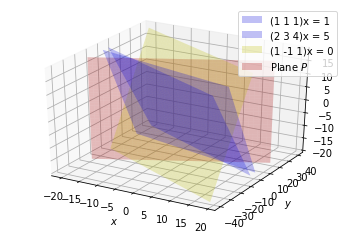
\includegraphics[ width=\columnwidth]{solutions/sep/2/28/figures/planes.png}
\caption{Plane $P$ passing through intersection of $P_{1}$ and $P_{2}$ and perpendicular to $P_{3}$}
\label{sep/2/28fig:Line }	
\end{figure}

%
\item In the following cases, determine whether the given planes are parallel or perpendicular, and in case they are neither, find the angles between them.
\begin{enumerate}
\item 
$
\myvec{7 & 5 & 6}\vec{x}=-30
$
 and 
$
\myvec{3 & -1 & -10}\vec{x}=-4
$
%
\item 
$
\myvec{2 & 1 & 3}\vec{x}=2
$
 and 
$
\myvec{1 & -2 & 5}\vec{x}=0
$
%
\item 
$
\myvec{2 & -2 & 4}\vec{x}=-5
$
 and 
$
\myvec{3 & -3 & 6}\vec{x}=1
$
\item 
$
\myvec{2 & -1 & 3}\vec{x}=1
$
 and 
$
\myvec{2 & -1 & 3}\vec{x}=-3
$
\item 
$
\myvec{4 & 8 & 1}\vec{x}=8
$
 and 
$
\myvec{0 & 1 & 1}\vec{x}=4
$
\end{enumerate}
\solution
\begin{enumerate}
    \item 
    
\begin{table}[!ht]
\centering
\resizebox{\columnwidth}{!}{\begin{tabular}{|c|c|c|c|} 
\hline
kind of  cake & No.of cakes & Flour& Fat\\
\hline
1st & x & 200g  &  25g \\ 
\hline
2nd& y& 100g&  50g  \\ 
\hline
Total& x+y& 5 kg=5000g&1kg=1000g \\ 
\hline
\end{tabular}}
\caption{Ingredients used in making the cake is flour and fat }
\label{opt/13/tab:table1}
\end{table}
Let the  1st kind  be $x$ and the 2nd kind be $y$  such that 
\begin{align}
x \geq 0 \\
y \geq 0 
\end{align}
According to the question,
\begin{align}
2{x} + {y} \leq 50
\\
{x} + 2{y} \leq 40
\end{align}
$\therefore$ Our problem is
\begin{align}
\max_{\vec{x}} Z &= \myvec{1& 1}\vec{x}\\
s.t. \quad \myvec{2 & 1 \\ 1& 2}\vec{x} &\preceq \myvec{50\\40} 
\end{align}
Lagrangian function is given by
\begin{equation}
\begin{aligned}
&L(\vec{x},\boldsymbol{\lambda}) \\ &= \myvec{1 & 1}\vec{x}+\lcbrak{\sbrak{\myvec{2 & 1}\vec{x}-50}} \\ &+ \sbrak{\myvec{1 & 2}\vec{x}-40}\\ &+ \sbrak{\myvec{-1 & 0}\vec{x}} +\rcbrak{\sbrak{\myvec{0 & -1}\vec{x}}}\boldsymbol{\lambda}
\end{aligned}
\end{equation}
where,
\begin{align}
\boldsymbol{\lambda} &= \myvec{\lambda_1 \\ \lambda_2 \\ \lambda_3 \\ \lambda_4 \\ \lambda_5 \\ \lambda_6}
\end{align}
Now,
\begin{align}
\nabla L(\vec{x},\boldsymbol{\lambda}) &= \myvec{1+ \myvec{2 & 1 & -1 & 0 }\boldsymbol{\lambda}\\ 1+\myvec{1 & 2 & 0 & -1}\boldsymbol{\lambda} \\ \myvec{2 & 1}\vec{x}-50\\ \myvec{1& 2}\vec{x}-40 \\  \myvec{-1 & 0}\vec{x} \\ \myvec{0 & -1}\vec{x}}
\end{align}
$\therefore$ Lagrangian matrix is given by
\begin{align}
\myvec{0 & 0 & 2 & 1& -1 & 0 \\ 0 & 0 & 1 & 2  & 0 & -1 \\ 2 & 1 & 0 & 0 & 0 & 0 \\ 1 & 2 & 0 & 0 & 0 & 0  \\ -1 & 0 & 0 & 0 & 0 & 0  \\ 0 & -1 & 0 & 0 & 0 & 0 }\myvec{\vec{x} \\ \boldsymbol{\lambda} } &= \myvec{-1 \\ -1 \\ 50\\ 4 0\\ 0 \\0 }
\end{align}
Considering $\lambda_1,\lambda_2$ as only active multiplier,
\begin{align}
\myvec{0 & 0 & 2 & 1 \\ 0 & 0 & 1 & 2 \\ 2 & 1 & 0 & 0 \\ 1 & 2 & 0 & 0}\myvec{\vec{x}\\ \boldsymbol{\lambda}} &= \myvec{-1 \\ -1 \\ 5 0\\ 40}
\end{align}
resulting in,
\begin{align}
\myvec{\vec{x} \\ \boldsymbol{\lambda}} &= \myvec{0 & 0 & 2 & 1 \\ 0 & 0 & 1 & 2 \\ 2 & 1 & 0 & 0 \\ 1& 2 & 0 & 0}^{-1}\myvec{-1 \\ -1 \\ 50 \\ 40}
\\
\implies   \myvec{\vec{x} \\ \boldsymbol{\lambda}} &= \myvec{0 & 0 & \frac{2}{3} & \frac{-1}{3} \\ 0 & 0 & \frac{-1}{3} & \frac{2}{3} \\ \frac{2}{3} & \frac{-1}{3} & 0 & 0 \\ \frac{-1}{3} & \frac{2}{3} & 0 & 0}\myvec{-1 \\ -1 \\ 50 \\ 40}
\\
\implies \myvec{\vec{x} \\ \boldsymbol{\lambda}} &= \myvec{20 \\ 10 \\ -0.3 \\ -0.3 }
\end{align}
$\because \boldsymbol{\lambda}=\myvec{-0.3 \\ -0.3} \succ \vec{0} $
\\
$\therefore$ Optimal solution is given by
\begin{align}
    \vec{x} &= \myvec{20\\10} \\
    Z &= \myvec{1& 1}\vec{x} \\
    &= \myvec{1 & 1}\myvec{20 \\ 10} \\
    &= 60
\end{align}
By using cvxpy in python ,
\begin{align}
    \vec{x}=\myvec{20\\10}\\
    Z = 60
\end{align}
Hence No.of cakes \boxed{x=20} 1st kind and  .of cakes \boxed{y=10} 2nd kind should be used to maximum No. of cakes \boxed{Z=60}.  This is
verified in Fig. \ref{opt/13/fig: Graphical Solution}.	
%
\begin{figure}[!ht]
\centering
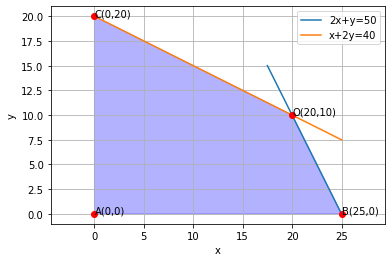
\includegraphics[width=\columnwidth]{solutions/su2021/2/13/Figure9.png}
\caption{Graphical Solution}
\label{opt/13/fig: Graphical Solution}	
\end{figure}

    \item 
    From the given information, 
\begin{equation}
 \vec n_1=\myvec{2\\-2\\4},
 \vec n_2 =\myvec{3\\-3\\6},
\end{equation}
and 
\begin{align}
    \theta &= \cos^{-1}\brak{{\frac{\vec{n}_1^{T}\vec{n}_2}{\norm{\vec{n_1}}\norm{\vec{n}_2}}}}
    \\
 &= 0\degree
\end{align}
Hence, the given planes are parallel, as can be seen from Fig. \ref{linform/43/c/fig: PARALLEL planes.}
%
\begin{figure}[ht]
    \centering
   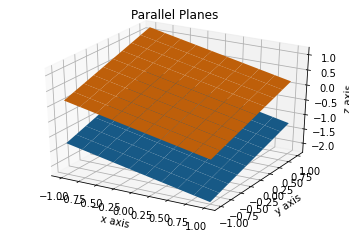
\includegraphics[width=\columnwidth]{solutions/su2021/2/43/c/ASSIGNMENT 5.png}
    \caption{Parallel planes}
    \label{linform/43/c/fig: PARALLEL planes.}
\end{figure}    

    \item 
    
\begin{table}[!ht]
\centering
\resizebox{\columnwidth}{!}{\begin{tabular}{|c|c|c|c|} 
\hline
kind of  cake & No.of cakes & Flour& Fat\\
\hline
1st & x & 200g  &  25g \\ 
\hline
2nd& y& 100g&  50g  \\ 
\hline
Total& x+y& 5 kg=5000g&1kg=1000g \\ 
\hline
\end{tabular}}
\caption{Ingredients used in making the cake is flour and fat }
\label{opt/13/tab:table1}
\end{table}
Let the  1st kind  be $x$ and the 2nd kind be $y$  such that 
\begin{align}
x \geq 0 \\
y \geq 0 
\end{align}
According to the question,
\begin{align}
2{x} + {y} \leq 50
\\
{x} + 2{y} \leq 40
\end{align}
$\therefore$ Our problem is
\begin{align}
\max_{\vec{x}} Z &= \myvec{1& 1}\vec{x}\\
s.t. \quad \myvec{2 & 1 \\ 1& 2}\vec{x} &\preceq \myvec{50\\40} 
\end{align}
Lagrangian function is given by
\begin{equation}
\begin{aligned}
&L(\vec{x},\boldsymbol{\lambda}) \\ &= \myvec{1 & 1}\vec{x}+\lcbrak{\sbrak{\myvec{2 & 1}\vec{x}-50}} \\ &+ \sbrak{\myvec{1 & 2}\vec{x}-40}\\ &+ \sbrak{\myvec{-1 & 0}\vec{x}} +\rcbrak{\sbrak{\myvec{0 & -1}\vec{x}}}\boldsymbol{\lambda}
\end{aligned}
\end{equation}
where,
\begin{align}
\boldsymbol{\lambda} &= \myvec{\lambda_1 \\ \lambda_2 \\ \lambda_3 \\ \lambda_4 \\ \lambda_5 \\ \lambda_6}
\end{align}
Now,
\begin{align}
\nabla L(\vec{x},\boldsymbol{\lambda}) &= \myvec{1+ \myvec{2 & 1 & -1 & 0 }\boldsymbol{\lambda}\\ 1+\myvec{1 & 2 & 0 & -1}\boldsymbol{\lambda} \\ \myvec{2 & 1}\vec{x}-50\\ \myvec{1& 2}\vec{x}-40 \\  \myvec{-1 & 0}\vec{x} \\ \myvec{0 & -1}\vec{x}}
\end{align}
$\therefore$ Lagrangian matrix is given by
\begin{align}
\myvec{0 & 0 & 2 & 1& -1 & 0 \\ 0 & 0 & 1 & 2  & 0 & -1 \\ 2 & 1 & 0 & 0 & 0 & 0 \\ 1 & 2 & 0 & 0 & 0 & 0  \\ -1 & 0 & 0 & 0 & 0 & 0  \\ 0 & -1 & 0 & 0 & 0 & 0 }\myvec{\vec{x} \\ \boldsymbol{\lambda} } &= \myvec{-1 \\ -1 \\ 50\\ 4 0\\ 0 \\0 }
\end{align}
Considering $\lambda_1,\lambda_2$ as only active multiplier,
\begin{align}
\myvec{0 & 0 & 2 & 1 \\ 0 & 0 & 1 & 2 \\ 2 & 1 & 0 & 0 \\ 1 & 2 & 0 & 0}\myvec{\vec{x}\\ \boldsymbol{\lambda}} &= \myvec{-1 \\ -1 \\ 5 0\\ 40}
\end{align}
resulting in,
\begin{align}
\myvec{\vec{x} \\ \boldsymbol{\lambda}} &= \myvec{0 & 0 & 2 & 1 \\ 0 & 0 & 1 & 2 \\ 2 & 1 & 0 & 0 \\ 1& 2 & 0 & 0}^{-1}\myvec{-1 \\ -1 \\ 50 \\ 40}
\\
\implies   \myvec{\vec{x} \\ \boldsymbol{\lambda}} &= \myvec{0 & 0 & \frac{2}{3} & \frac{-1}{3} \\ 0 & 0 & \frac{-1}{3} & \frac{2}{3} \\ \frac{2}{3} & \frac{-1}{3} & 0 & 0 \\ \frac{-1}{3} & \frac{2}{3} & 0 & 0}\myvec{-1 \\ -1 \\ 50 \\ 40}
\\
\implies \myvec{\vec{x} \\ \boldsymbol{\lambda}} &= \myvec{20 \\ 10 \\ -0.3 \\ -0.3 }
\end{align}
$\because \boldsymbol{\lambda}=\myvec{-0.3 \\ -0.3} \succ \vec{0} $
\\
$\therefore$ Optimal solution is given by
\begin{align}
    \vec{x} &= \myvec{20\\10} \\
    Z &= \myvec{1& 1}\vec{x} \\
    &= \myvec{1 & 1}\myvec{20 \\ 10} \\
    &= 60
\end{align}
By using cvxpy in python ,
\begin{align}
    \vec{x}=\myvec{20\\10}\\
    Z = 60
\end{align}
Hence No.of cakes \boxed{x=20} 1st kind and  .of cakes \boxed{y=10} 2nd kind should be used to maximum No. of cakes \boxed{Z=60}.  This is
verified in Fig. \ref{opt/13/fig: Graphical Solution}.	
%
\begin{figure}[!ht]
\centering
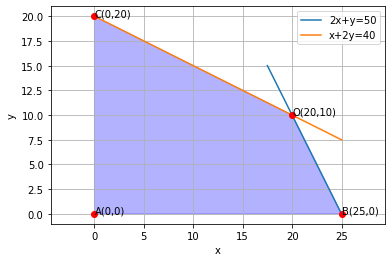
\includegraphics[width=\columnwidth]{solutions/su2021/2/13/Figure9.png}
\caption{Graphical Solution}
\label{opt/13/fig: Graphical Solution}	
\end{figure}

    %
\end{enumerate}
\item In the following cases, find the distance of each of the given points from the corresponding plane.
%\newcounter{rowno}
%\setcounter{rowno}{0}
\begin{table}[!h]
\centering
%\begin{tabular}{>{\stepcounter{rowno}\therowno.}cl}
%\multicolumn{1}{r}{No.} & text & abcd\\\hline
% & first  \\
% & second \\
% & third  \\
% & fourth 
%\end{tabular}
%%%%%%%%%%%%%%%%%%%%%%%%%%%%%%%%%%%%%%%%%%%%%%%%%%%%%%%%%%%%%%%%%%%%%%
%%                                                                  %%
%%  This is the header of a LaTeX2e file exported from Gnumeric.    %%
%%                                                                  %%
%%  This file can be compiled as it stands or included in another   %%
%%  LaTeX document. The table is based on the longtable package so  %%
%%  the longtable options (headers, footers...) can be set in the   %%
%%  preamble section below (see PRAMBLE).                           %%
%%                                                                  %%
%%  To include the file in another, the following two lines must be %%
%%  in the including file:                                          %%
%%        \def\inputGnumericTable{}                                 %%
%%  at the beginning of the file and:                               %%
%%        \input{name-of-this-file.tex}                             %%
%%  where the table is to be placed. Note also that the including   %%
%%  file must use the following packages for the table to be        %%
%%  rendered correctly:                                             %%
%%    \usepackage[latin1]{inputenc}                                 %%
%%    \usepackage{color}                                            %%
%%    \usepackage{array}                                            %%
%%    \usepackage{longtable}                                        %%
%%    \usepackage{calc}                                             %%
%%    \usepackage{multirow}                                         %%
%%    \usepackage{hhline}                                           %%
%%    \usepackage{ifthen}                                           %%
%%  optionally (for landscape tables embedded in another document): %%
%%    \usepackage{lscape}                                           %%
%%                                                                  %%
%%%%%%%%%%%%%%%%%%%%%%%%%%%%%%%%%%%%%%%%%%%%%%%%%%%%%%%%%%%%%%%%%%%%%%



%%  This section checks if we are begin input into another file or  %%
%%  the file will be compiled alone. First use a macro taken from   %%
%%  the TeXbook ex 7.7 (suggestion of Han-Wen Nienhuys).            %%
\def\ifundefined#1{\expandafter\ifx\csname#1\endcsname\relax}


%%  Check for the \def token for inputed files. If it is not        %%
%%  defined, the file will be processed as a standalone and the     %%
%%  preamble will be used.                                          %%
\ifundefined{inputGnumericTable}

%%  We must be able to close or not the document at the end.        %%
	\def\gnumericTableEnd{\end{document}}


%%%%%%%%%%%%%%%%%%%%%%%%%%%%%%%%%%%%%%%%%%%%%%%%%%%%%%%%%%%%%%%%%%%%%%
%%                                                                  %%
%%  This is the PREAMBLE. Change these values to get the right      %%
%%  paper size and other niceties.                                  %%
%%                                                                  %%
%%%%%%%%%%%%%%%%%%%%%%%%%%%%%%%%%%%%%%%%%%%%%%%%%%%%%%%%%%%%%%%%%%%%%%

	\documentclass[12pt%
			  %,landscape%
                    ]{report}
       \usepackage[latin1]{inputenc}
       \usepackage{fullpage}
       \usepackage{color}
       \usepackage{array}
       \usepackage{longtable}
       \usepackage{calc}
       \usepackage{multirow}
       \usepackage{hhline}
       \usepackage{ifthen}

	\begin{document}


%%  End of the preamble for the standalone. The next section is for %%
%%  documents which are included into other LaTeX2e files.          %%
\else

%%  We are not a stand alone document. For a regular table, we will %%
%%  have no preamble and only define the closing to mean nothing.   %%
    \def\gnumericTableEnd{}

%%  If we want landscape mode in an embedded document, comment out  %%
%%  the line above and uncomment the two below. The table will      %%
%%  begin on a new page and run in landscape mode.                  %%
%       \def\gnumericTableEnd{\end{landscape}}
%       \begin{landscape}


%%  End of the else clause for this file being \input.              %%
\fi

%%%%%%%%%%%%%%%%%%%%%%%%%%%%%%%%%%%%%%%%%%%%%%%%%%%%%%%%%%%%%%%%%%%%%%
%%                                                                  %%
%%  The rest is the gnumeric table, except for the closing          %%
%%  statement. Changes below will alter the table's appearance.     %%
%%                                                                  %%
%%%%%%%%%%%%%%%%%%%%%%%%%%%%%%%%%%%%%%%%%%%%%%%%%%%%%%%%%%%%%%%%%%%%%%

\providecommand{\gnumericmathit}[1]{#1} 
%%  Uncomment the next line if you would like your numbers to be in %%
%%  italics if they are italizised in the gnumeric table.           %%
%\renewcommand{\gnumericmathit}[1]{\mathit{#1}}
\providecommand{\gnumericPB}[1]%
{\let\gnumericTemp=\\#1\let\\=\gnumericTemp\hspace{0pt}}
 \ifundefined{gnumericTableWidthDefined}
        \newlength{\gnumericTableWidth}
        \newlength{\gnumericTableWidthComplete}
        \newlength{\gnumericMultiRowLength}
        \global\def\gnumericTableWidthDefined{}
 \fi
%% The following setting protects this code from babel shorthands.  %%
 \ifthenelse{\isundefined{\languageshorthands}}{}{\languageshorthands{english}}
%%  The default table format retains the relative column widths of  %%
%%  gnumeric. They can easily be changed to c, r or l. In that case %%
%%  you may want to comment out the next line and uncomment the one %%
%%  thereafter                                                      %%
\providecommand\gnumbox{\makebox[0pt]}
%%\providecommand\gnumbox[1][]{\makebox}

%% to adjust positions in multirow situations                       %%
\setlength{\bigstrutjot}{\jot}
\setlength{\extrarowheight}{\doublerulesep}

%%  The \setlongtables command keeps column widths the same across  %%
%%  pages. Simply comment out next line for varying column widths.  %%
\setlongtables

\setlength\gnumericTableWidth{%
	44pt+%
	44pt+%
	84pt+%
0pt}
\def\gumericNumCols{3}
\setlength\gnumericTableWidthComplete{\gnumericTableWidth+%
         \tabcolsep*\gumericNumCols*2+\arrayrulewidth*\gumericNumCols}
\ifthenelse{\lengthtest{\gnumericTableWidthComplete > \linewidth}}%
         {\def\gnumericScale{\ratio{\linewidth-%
                        \tabcolsep*\gumericNumCols*2-%
                        \arrayrulewidth*\gumericNumCols}%
{\gnumericTableWidth}}}%
{\def\gnumericScale{1}}

%%%%%%%%%%%%%%%%%%%%%%%%%%%%%%%%%%%%%%%%%%%%%%%%%%%%%%%%%%%%%%%%%%%%%%
%%                                                                  %%
%% The following are the widths of the various columns. We are      %%
%% defining them here because then they are easier to change.       %%
%% Depending on the cell formats we may use them more than once.    %%
%%                                                                  %%
%%%%%%%%%%%%%%%%%%%%%%%%%%%%%%%%%%%%%%%%%%%%%%%%%%%%%%%%%%%%%%%%%%%%%%

\ifthenelse{\isundefined{\gnumericColA}}{\newlength{\gnumericColA}}{}\settowidth{\gnumericColA}{\begin{tabular}{@{}p{44pt*\gnumericScale}@{}}x\end{tabular}}
\ifthenelse{\isundefined{\gnumericColB}}{\newlength{\gnumericColB}}{}\settowidth{\gnumericColB}{\begin{tabular}{@{}p{44pt*\gnumericScale}@{}}x\end{tabular}}
\ifthenelse{\isundefined{\gnumericColC}}{\newlength{\gnumericColC}}{}\settowidth{\gnumericColC}{\begin{tabular}{@{}p{84pt*\gnumericScale}@{}}x\end{tabular}}


\begin{tabular}[c]{%
	b{\gnumericColA}%
	b{\gnumericColB}%
	b{\gnumericColC}%
	}

%%%%%%%%%%%%%%%%%%%%%%%%%%%%%%%%%%%%%%%%%%%%%%%%%%%%%%%%%%%%%%%%%%%%%%
%%  The longtable options. (Caption, headers... see Goosens, p.124) %%
%	\caption{The Table Caption.}             \\	%
% \hline	% Across the top of the table.
%%  The rest of these options are table rows which are placed on    %%
%%  the first, last or every page. Use \multicolumn if you want.    %%

%%  Header for the first page.                                      %%
%	\multicolumn{3}{c}{The First Header} \\ \hline 
%	\multicolumn{1}{c}{colTag}	%Column 1
%	&\multicolumn{1}{c}{colTag}	%Column 2
%	&\multicolumn{1}{c}{colTag}	\\ \hline %Last column
%	\endfirsthead

%%  The running header definition.                                  %%
%	\hline
%	\multicolumn{3}{l}{\ldots\small\slshape continued} \\ \hline
%	\multicolumn{1}{c}{colTag}	%Column 1
%	&\multicolumn{1}{c}{colTag}	%Column 2
%	&\multicolumn{1}{c}{colTag}	\\ \hline %Last column
%	\endhead

%%  The running footer definition.                                  %%
%	\hline
%	\multicolumn{3}{r}{\small\slshape continued\ldots} \\
%	\endfoot

%%  The ending footer definition.                                   %%
%	\multicolumn{3}{c}{That's all folks} \\ \hline 
%	\endlastfoot
%%%%%%%%%%%%%%%%%%%%%%%%%%%%%%%%%%%%%%%%%%%%%%%%%%%%%%%%%%%%%%%%%%%%%%

\hhline{|-|-|-}
	 \multicolumn{1}{|p{\gnumericColA}|}%
	{\gnumericPB{\centering}\gnumbox{\textbf{Item}}}
	&\multicolumn{1}{p{\gnumericColB}|}%
	{\gnumericPB{\centering}\gnumbox{\textbf{Point}}}
	&\multicolumn{1}{p{\gnumericColC}|}%
	{\gnumericPB{\centering}\gnumbox{\textbf{Plane}}}
\\
\hhline{|---|}
	 \multicolumn{1}{|p{\gnumericColA}|}%
	{a)}
	&\multicolumn{1}{p{\gnumericColB}|}%
	{\gnumericPB{\centering}\gnumbox{\myvec{0\\0\\0}}}
	&\multicolumn{1}{p{\gnumericColC}|}%
	{\gnumericPB{\centering}\gnumbox{$\myvec{3 & -4 & 12}\bm{x}=3$}}
\\
\hhline{|---|}
	 \multicolumn{1}{|p{\gnumericColA}|}%
	{b)}
	&\multicolumn{1}{p{\gnumericColB}|}%
	{\gnumericPB{\centering}\gnumbox{\myvec{3\\-2\\1}}}
	&\multicolumn{1}{p{\gnumericColC}|}%
	{\gnumericPB{\centering}\gnumbox{$\myvec{2 & -1 & 2}\bm{x}=-3$}}
\\
\hhline{|---|}
	 \multicolumn{1}{|p{\gnumericColA}|}%
	{c)}
	&\multicolumn{1}{p{\gnumericColB}|}%
	{\gnumericPB{\centering}\gnumbox{\myvec{2\\3\\-5}}}
	&\multicolumn{1}{p{\gnumericColC}|}%
	{\gnumericPB{\centering}\gnumbox{$\myvec{1 & 2 & -2}\bm{x}=9$}}
\\
\hhline{|---|}
	 \multicolumn{1}{|p{\gnumericColA}|}%
	{d)}
	&\multicolumn{1}{p{\gnumericColB}|}%
	{\gnumericPB{\centering}\gnumbox{\myvec{-6\\0\\0}}}
	&\multicolumn{1}{p{\gnumericColC}|}%
	{\gnumericPB{\centering}\gnumbox{$\myvec{2 & -3 & 6}\bm{x}=2$}}
\\
\hhline{|-|-|-|}
\end{tabular}

\ifthenelse{\isundefined{\languageshorthands}}{}{\languageshorthands{\languagename}}
\gnumericTableEnd

\caption{}
\label{table:3d}
\end{table}
%
\item 
\item 
\item If the lines 
\begin{align}
\frac{x-1}{-3} = \frac{y-2}{2k} &= \frac{z-3}{2}, 
\\
\frac{x-3}{3k} = \frac{y-1}{1} &= \frac{z-6}{-5} ,
\end{align}
find the value of $k$.
\item Find the  equation of the line passing through \myvec{1\\2\\3} and perpendicular to the plane %
\begin{align}
\myvec{1 & 2 & -5}\vec{x}&=-9
\end{align}
\solution

Let $\vec{p} = \myvec{1\\2\\3}$ be a point on the line L.
Direction vector of the  line perpendicular to the given plane is
\begin{align}
 \myvec{1\\2\\-5}
\end{align}
Thus, the equation of required line is
\begin{align}
    L: \quad \vec{x}&=\vec{p}+\lambda\vec{a}\\ &=\myvec{1\\2\\3}+\lambda\myvec{1\\2\\-5}
\end{align}
See Fig.  \ref{aug/2/34/plot}.
\begin{figure}[!h]
 \centering
 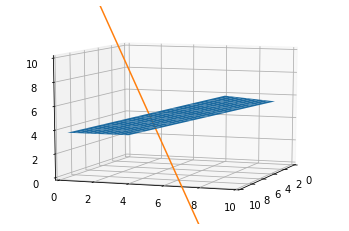
\includegraphics[width=\columnwidth]{solutions/aug/2/34/figs/Assignment4.png}
 \caption{Plot of plane and the line}
 \label{aug/2/34/plot}
\end{figure}



\item Find the shortest distance between the lines 
%
\begin{align}
\vec{x} = \myvec{6 \\ 2 \\ 2} + \lambda_1 \myvec{1 \\ -2 \\ 2}  \text{ and }
\\
\vec{x} = \myvec{-4 \\ 0 \\ -1} + \lambda_2 \myvec{3 \\ -2 \\ -2}  
\end{align}
%
\item Find the coordinates of the point where the line through \myvec{5\\1\\6} and \myvec{3\\4\\1} crosses the YZ-plane.
\\
\solution
% The equation of a plane $P$ passing through the line of intersection of the planes $P_{1}$ and $P_{2}$ has the form,
% \begin{align}
%    P : P_{1} + \lambda P_{2}\label{sep/2/28eq1}
% \end{align}
% %
% General equation of plane is given by
% \begin{align}
%     \vec{n}^T\vec{x}=c
% \end{align}
% Where $\vec{n}$ is normal vector to the plane
\begin{lemma}
   The equation of a plane passing through intersection of planes
   \begin{align}
    \vec{n_{1}}^T\vec{x}&=c_{1}\\ \vec{n_{2}}^T\vec{x}&=c_{2}
   \end{align}
   and perpendicular to plane
   \begin{align}
     \vec{n_{3}}^T\vec{x}&=c_{3}
   \end{align}
   is given by 
   \begin{align}
      \vec{n_{4}}^T\vec{x}&=c_{4}
   \end{align}
   where 
   \begin{align}
       \vec{n_{4}} = \vec{n_{1}} - \brak{\frac{\vec{n_{3}^T\vec{n_1}}}{\vec{n_{3}^T\vec{n_2}}}}\vec{n_2}\\
       c_{4} = c_{1} - \brak{\frac{\vec{n_{3}^T\vec{n_1}}}{\vec{n_{3}^T\vec{n_2}}}}c_{2}
   \end{align}
\end{lemma}
\begin{proof}
   Let $P$ be the plane that passes through intersection 2 given planes.\\  From \eqref{sep/2/28/eq1}, equation of $P$ has the form,
   \begin{align}
       \vec{n_{1}}^T\vec{x} + \lambda\brak{\vec{n_{2}}^T\vec{x}} = c_{1} + \lambda\brak{c_{2}}\\
       \implies \brak{\vec{n_{1}}+\lambda\vec{n_{2}}}^T\vec{x} = c_{1} + \lambda\brak{c_{2}}
   \end{align}
  Normal vector to plane $P$ is,
 \begin{align}
     \vec{n_{4}} = \vec{n_{1}}+\lambda\vec{n_{2}}
 \end{align}
 As $P$ is perpendicular to the third plane i.e. angle between normal vectors is $90\degree$, 
 \begin{align}
     &\cos\brak{90\degree} = 0 = \dfrac{\vec{n_{3}}^T\vec{n_{4}}}{\norm{\vec{n_{3}}}\norm{\vec{n_{4}}}}\\
    \implies &\vec{n_{3}}^T\vec{n_{4}} = 0\\
    \implies &\vec{n_{3}}^T\brak{\vec{n_{1}}+\lambda\vec{n_{2}}} = 0\\
    \implies &\lambda = \frac{-\vec{n_{3}^T\vec{n_1}}}{\vec{n_{3}^T\vec{n_2}}}
 \end{align}
 Therefore equation of plane $P$ is,
 \begin{align}
     \brak{\vec{n_{1}} - \brak{\frac{\vec{n_{3}^T\vec{n_1}}}{\vec{n_{3}^T\vec{n_2}}}}\vec{n_2}}^T\vec{x} = c_{1} - \brak{\frac{\vec{n_{3}^T\vec{n_1}}}{\vec{n_{3}^T\vec{n_2}}}}c_{2}
 \end{align}
\end{proof}
For the given problem,
\begin{align}
  \vec{n_{1}}=\myvec{1\\1\\1}\\c_{1}=1,
  \vec{n_{2}}=\myvec{2\\3\\4},
     c_{2}=5\\
  \vec{n_{3}}=\myvec{1\\-1\\1}\\c_{3}=0 
 \end{align}
Solving the above we get,
\begin{align}
    \lambda = \frac{-1}{3},
    \vec{n_{4}} = \myvec{\frac{1}{3}\\0\\\frac{-1}{3}},
    c_{4} = \frac{-2}{3}
\end{align}
We have equation of the plane as,
\begin{align}
    \myvec{\frac{1}{3}&0&\frac{-1}{3}}\vec{x} = \frac{-2}{3} 
\end{align}
\begin{figure}[!ht]
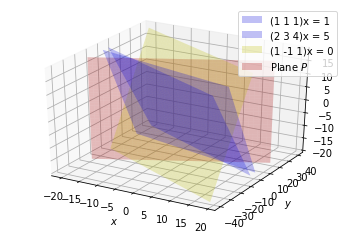
\includegraphics[ width=\columnwidth]{solutions/sep/2/28/figures/planes.png}
\caption{Plane $P$ passing through intersection of $P_{1}$ and $P_{2}$ and perpendicular to $P_{3}$}
\label{sep/2/28fig:Line }	
\end{figure}


\item Find the coordinates of the point where the line through \myvec{5\\1\\6} and \myvec{3\\4\\1} crosses the ZX-plane.
\\
\solution
Let the equation of line be
\begin{align}
    \vec{n}^\top\brak{\vec{x}-\vec{P}}=0
\end{align}
So the perpendicular from the origin meets the line at $\vec{P}= \myvec{-2 \\ 9}$.Since,
\begin{align}
   \vec{n}&= \vec{P}-\vec{O}\\
   &=\myvec{-2-0\\9-0}\\
   &=\myvec{-2\\9}
\end{align}
is the normal vector where $\vec{O}$ is the origin then 
is the direction vector, Hence the equation of line is given by
\begin{align}
   \myvec{-2 & 9}\brak{\vec{x}-\myvec{-2 \\ 9}}&=0 \\
\implies     \myvec{-2 & 9}\vec{x}&= 85
\end{align}
    See Fig. \ref{aug/2/21/fig:my_label}
\begin{figure}[htp]
    \centering
    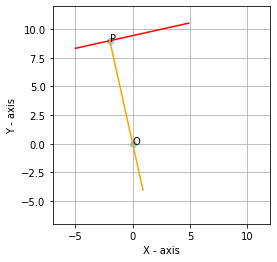
\includegraphics{solutions/aug/2/21/Assignment_4.png}
    \caption{graph}
    \label{aug/2/21/fig:my_label}
\end{figure}


%
\item Find the equation of the plane passing through the point \myvec{-1\\3\\2} and perpendicular to each of the planes 
\begin{align}
\myvec{1 & 2 & 3}\vec{x}&=5
\\
\myvec{3 & 3 & 1}\vec{x}&=0
\end{align}
\item If the points \myvec{1\\1\\p} and \myvec{-3\\0\\1} be equidistant from the plane 
\begin{align}
\myvec{3 & 4 & -12}\vec{x}&=-13,
\end{align}
%
then find the value of $p$.
\item Find the equation of the plane passing through the line of intersection of the planes 
\begin{align}
\myvec{1 & 1 & 1}\vec{x}&=1 \text{ and }
\\
\myvec{2 & 3 & -1}\vec{x}&=-4
\end{align}
%
and parallel to the x-axis.
%
\\
\solution

\begin{table}[!ht]
\centering
\resizebox{\columnwidth}{!}{\begin{tabular}{|c|c|c|c|} 
\hline
kind of  cake & No.of cakes & Flour& Fat\\
\hline
1st & x & 200g  &  25g \\ 
\hline
2nd& y& 100g&  50g  \\ 
\hline
Total& x+y& 5 kg=5000g&1kg=1000g \\ 
\hline
\end{tabular}}
\caption{Ingredients used in making the cake is flour and fat }
\label{opt/13/tab:table1}
\end{table}
Let the  1st kind  be $x$ and the 2nd kind be $y$  such that 
\begin{align}
x \geq 0 \\
y \geq 0 
\end{align}
According to the question,
\begin{align}
2{x} + {y} \leq 50
\\
{x} + 2{y} \leq 40
\end{align}
$\therefore$ Our problem is
\begin{align}
\max_{\vec{x}} Z &= \myvec{1& 1}\vec{x}\\
s.t. \quad \myvec{2 & 1 \\ 1& 2}\vec{x} &\preceq \myvec{50\\40} 
\end{align}
Lagrangian function is given by
\begin{equation}
\begin{aligned}
&L(\vec{x},\boldsymbol{\lambda}) \\ &= \myvec{1 & 1}\vec{x}+\lcbrak{\sbrak{\myvec{2 & 1}\vec{x}-50}} \\ &+ \sbrak{\myvec{1 & 2}\vec{x}-40}\\ &+ \sbrak{\myvec{-1 & 0}\vec{x}} +\rcbrak{\sbrak{\myvec{0 & -1}\vec{x}}}\boldsymbol{\lambda}
\end{aligned}
\end{equation}
where,
\begin{align}
\boldsymbol{\lambda} &= \myvec{\lambda_1 \\ \lambda_2 \\ \lambda_3 \\ \lambda_4 \\ \lambda_5 \\ \lambda_6}
\end{align}
Now,
\begin{align}
\nabla L(\vec{x},\boldsymbol{\lambda}) &= \myvec{1+ \myvec{2 & 1 & -1 & 0 }\boldsymbol{\lambda}\\ 1+\myvec{1 & 2 & 0 & -1}\boldsymbol{\lambda} \\ \myvec{2 & 1}\vec{x}-50\\ \myvec{1& 2}\vec{x}-40 \\  \myvec{-1 & 0}\vec{x} \\ \myvec{0 & -1}\vec{x}}
\end{align}
$\therefore$ Lagrangian matrix is given by
\begin{align}
\myvec{0 & 0 & 2 & 1& -1 & 0 \\ 0 & 0 & 1 & 2  & 0 & -1 \\ 2 & 1 & 0 & 0 & 0 & 0 \\ 1 & 2 & 0 & 0 & 0 & 0  \\ -1 & 0 & 0 & 0 & 0 & 0  \\ 0 & -1 & 0 & 0 & 0 & 0 }\myvec{\vec{x} \\ \boldsymbol{\lambda} } &= \myvec{-1 \\ -1 \\ 50\\ 4 0\\ 0 \\0 }
\end{align}
Considering $\lambda_1,\lambda_2$ as only active multiplier,
\begin{align}
\myvec{0 & 0 & 2 & 1 \\ 0 & 0 & 1 & 2 \\ 2 & 1 & 0 & 0 \\ 1 & 2 & 0 & 0}\myvec{\vec{x}\\ \boldsymbol{\lambda}} &= \myvec{-1 \\ -1 \\ 5 0\\ 40}
\end{align}
resulting in,
\begin{align}
\myvec{\vec{x} \\ \boldsymbol{\lambda}} &= \myvec{0 & 0 & 2 & 1 \\ 0 & 0 & 1 & 2 \\ 2 & 1 & 0 & 0 \\ 1& 2 & 0 & 0}^{-1}\myvec{-1 \\ -1 \\ 50 \\ 40}
\\
\implies   \myvec{\vec{x} \\ \boldsymbol{\lambda}} &= \myvec{0 & 0 & \frac{2}{3} & \frac{-1}{3} \\ 0 & 0 & \frac{-1}{3} & \frac{2}{3} \\ \frac{2}{3} & \frac{-1}{3} & 0 & 0 \\ \frac{-1}{3} & \frac{2}{3} & 0 & 0}\myvec{-1 \\ -1 \\ 50 \\ 40}
\\
\implies \myvec{\vec{x} \\ \boldsymbol{\lambda}} &= \myvec{20 \\ 10 \\ -0.3 \\ -0.3 }
\end{align}
$\because \boldsymbol{\lambda}=\myvec{-0.3 \\ -0.3} \succ \vec{0} $
\\
$\therefore$ Optimal solution is given by
\begin{align}
    \vec{x} &= \myvec{20\\10} \\
    Z &= \myvec{1& 1}\vec{x} \\
    &= \myvec{1 & 1}\myvec{20 \\ 10} \\
    &= 60
\end{align}
By using cvxpy in python ,
\begin{align}
    \vec{x}=\myvec{20\\10}\\
    Z = 60
\end{align}
Hence No.of cakes \boxed{x=20} 1st kind and  .of cakes \boxed{y=10} 2nd kind should be used to maximum No. of cakes \boxed{Z=60}.  This is
verified in Fig. \ref{opt/13/fig: Graphical Solution}.	
%
\begin{figure}[!ht]
\centering
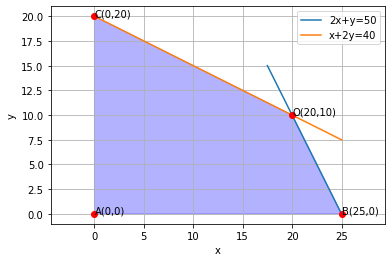
\includegraphics[width=\columnwidth]{solutions/su2021/2/13/Figure9.png}
\caption{Graphical Solution}
\label{opt/13/fig: Graphical Solution}	
\end{figure}

\item Find the equation of the plane which contains the line of intersection of the planes 
%
\begin{align}
\myvec{1 & 2 & 3}\vec{x}&=4 
\\
\myvec{2 & 1 & -1}\vec{x}&=-5
\end{align}
%
and which is perpendicular to the plane 
\begin{align}
\myvec{5 & 3 & -6}\vec{x}&=-8
\end{align}
%
\item Find the vector equation of the line passing through \myvec{1\\2\\3} and parallel to the planes 
%
\begin{align}
\myvec{1 & -1 & 2}\vec{x}&=5
\\
\myvec{3 & 1 & 1}\vec{x}&=6
\end{align}
%
\solution
%The normal vector to the desired plane is perpendicular the normal vectors of both the given planes. Thus
\begin{align}
\vec{n}&=\vec{n_1} \times \vec{n_2}
\\
&=\myvec{1\\-1\\2} \times \myvec{3\\1\\1}\\=\myvec{-3\\5\\4}
\end{align}
and the equation of the line is
\begin{align}
\vec{r}=\myvec{1\\2\\3}+\lambda \myvec{-3\\5\\4}   
\end{align}

\item The planes 
%
\begin{align}
\myvec{2 & -1 & 4}\vec{x}&=5
\\
\myvec{5 & -\frac{5}{2} & 10}\vec{x}&=6
\end{align}
%
are 
%
\begin{enumerate}[itemsep=2pt]
\begin{multicols}{2}
\item Perpendicular
\item Parallel
\item intersect y-axis
\item passes through $\myvec{0\\0\\\frac{5}{4}}$
\end{multicols}
\end{enumerate}
%
\item Find the maximum and minimum values, if any of
the following functions given by 
%
\begin{enumerate}
\item $f(x) = \abs{x+2}-1$
\item $f(x) = -\abs{x+1}+3$
\item $h(x) = x+1, x \in \brak{-1,1}$.
\end{enumerate}
%
\item Using integration find the area of region bounded by the triangle whose vertices are \myvec{1\\ 0}, \myvec{2\\ 2} and \myvec{3\\ 1}.
%
\item  Using integration find the area of region bounded by the triangle whose vertices are (– 1, 0), (1, 3) and (3, 2).
\item  Using integration find the area of the triangular region whose sides have the equations $\myvec{2 & -1 }\vec{x} = -1$, $\myvec{3 & -1 }\vec{x} = -1$ and x = 4.
%
\item Find the area of the region bounded by the line $\myvec{3 & -1}\vec{x} = -2$, the x-axis and the ordinates $x = -1, x = 1$.
\item Find the area bounded by the curve $\abs{x}+\abs{y} = 1$.
\item Using the method of integration find the area of $\triangle ABC$, whose vertices are $\vec{A} = \myvec{ 2\\0 }, \vec{B} = \myvec{ 4\\5 }, \vec{C} = \myvec{ 6\\3 }$.
\item  Using integration find the area of the triangular region whose sides have the equations $\myvec{2 & 1 }\vec{x} = 4$, $\myvec{3 & -2 }\vec{x} = 6$ and  $\myvec{1 & -3 }\vec{x} = -5$.
\item The two equal sides of an isosceles triangle with fixed base $b$ are decreasing at the rate of 3 cm per second. How fast is the area decreasing when the two equal sides are equal to the base ?
\item A tank with rectangular base and rectangular sides, open at the top is to be constructed so that its depth is 2 m and volume is 8 $m^3$
. If building of tank costs
\rupee 70 per sq metres for the base and Rs 45 per square metre for sides. What is the cost of least expensive tank?
\item A point on the hypotenuse of a triangle is at distance a and b from the sides of the triangle.
Show that the minimum length of the hypotenuse is
%
\begin{align}
\brak{a^{\frac{2}{3}}+b^{\frac{2}{3}}}^{\frac{3}{2}}
\end{align}
%
\item Prove that the function $f(x) = 5x – 3$ is continuous at $x = 0, at x = – 3$ and at $x = 5$.
\item Examine the following functions for continuity.
%
\begin{enumerate}
\item $f(x) = x-5$
\item $f(x) = \abs{x-1}$
\end{enumerate}
%
\item Is the function defined by 
%
\begin{align}
f(x)=
\begin{cases}
x, & x \le 1,
\\
5, & x > 1
\end{cases}
\end{align}
%
continuous at $x = 0$? At $x = 1$? At $x = 2$?
\item Find all points of discontinuity of $f$, where $f$ is defined by
%
\begin{enumerate}
\item 
$
\begin{alignedat}[t]{2}
f(x)=
\begin{cases}
2x+3, & x \le 2,
\\
2x-3, & x > 2
\end{cases}
\end{alignedat}
$
%
\item 
$
\begin{alignedat}[t]{2}
f(x)=
\begin{cases}
\abs{x}+3, & x \le -3,
\\
-2x, & -3 < x < 3
\\
6x+2, & x \ge 2
\end{cases}
\end{alignedat}
$
\item 
$
\begin{alignedat}[t]{2}
f(x)=
\begin{cases}
\frac{\abs{x}}{x}, & x \ne 0,
\\
0, & x = 0,
\end{cases}
\end{alignedat}
$
\item 
$
\begin{alignedat}[t]{2}
f(x)=
\begin{cases}
\frac{x}{\abs{x}}, & x < 0,
\\
-1, & x \ge 0,
\end{cases}
\end{alignedat}
$
\end{enumerate}
%
\item Is the function defined by 
%
\begin{align}
f(x)=
\begin{cases}
x+5, & x \le 1,
\\
x-5, & x > 1
\end{cases}
\end{align}
%
a continuous function?
\item Discuss the continuity of the function $f$, where $f$ is defined by 
\begin{enumerate}
\item 
$
\begin{alignedat}[t]{2}
f(x)=
\begin{cases}
3, & 0 \le x \le 1,
\\
4, & 0 < x \le 3,
\\
5, & 3 \le x \le 10,
\end{cases}
\end{alignedat}
$
%
\item 
$
\begin{alignedat}[t]{2}
f(x)=
\begin{cases}
2x, & x < 0,
\\
0, & 0 \le x \le 1
\\
4x, &  x > 1
\end{cases}
\end{alignedat}
$
\item 
$
\begin{alignedat}[t]{2}
f(x)=
\begin{cases}
-2, & x < -1,
\\
2x, & -1 \le x \le  1
\\
2, & x >  1
\end{cases}
\end{alignedat}
$
\end{enumerate}
%
\item Find the relationship between $a$ and $b$ so that the function defined by 	
%
\begin{align}
f(x)=
\begin{cases}
ax+1, & x \le 3,
\\
bx+3, & x > 3
\end{cases}
\end{align}
%
is continuous at $x = 3$
%
\item Prove that the function $f(x) = x$ is continuious at every real number.
\item Is $f(x) = \abs{x}$ a continuous function?
\item Discuss the continuity of the function $f$ defined by 
%
\begin{align}
f(x)  = 
\begin{cases}
x+2 & x \le 1
\\
x-2 & x > 1
\end{cases}
\end{align}

\item Show that the function defined by $g (x) = x – [x]$ is discontinuous at all integral points. Here $[x]$ denotes the greatest integer less than or equal to $x$.
\item For what value of $k$ is the following function 
%
continuous at the given point.
\begin{align}
f(x)=
\begin{cases}
kx+1, & x \le 5,
\\
3x-5, & x > 5,
\end{cases}
\quad x = 5
\end{align}
\item Prove that the function $f$ given by 
\begin{align}
f(x) = \abs{x-1}, x \in \vec{R}
\end{align}
%
is not differentiable at $x = 1$.
\item Prove that the greatest integer function defined by 
\begin{align}
f(x) = \abs{x}, 0 < x < 3
\end{align}
%
is not differentiable at $x = 1$ and $x = 2$.
\item Examine if Rolle's theorem is applicable to the following functions
\begin{enumerate}
\item 
\label{prob:line_eq_rolle}
$
f(x) = \sbrak{x}, x \in \sbrak{5,9}.
$
\item 
$
f(x) = \sbrak{x}, x \in \sbrak{-2,2}.
$
\end{enumerate}
Can you say some thing about the converse of Rolle's theorem from this example?
\item  Examine the applicability of the mean value theorem for all functions in Problem \ref{prob:line_eq_rolle}.
%
\item Find $\lim_{x\to 5} x+10$
\item Find $\lim_{x\to 2} 3x$
\item Find $\lim_{x\to 0}f(x)$ where
%
\begin{align}
f(x)  = 
\begin{cases}
1 & x \le 0
\\
2 & x > 0
\end{cases}
\end{align}
\item Find $\lim_{x\to 0}f(x)$ where
%
\begin{align}
f(x)  = 
\begin{cases}
x-2 & x < 0
\\
0 & x = 0
\\
x+2 & x > 0
\end{cases}
\end{align}
\item Evaluate the following limits
\begin{enumerate}
\item $\lim_{x\to 3}x+3$
\item $\lim_{x\to \pi}\brak{x-\frac{22}{7}}$
\end{enumerate}
%
\item Find $\lim_{x\to 0} f(x)$ where
\begin{align}
f(x) = 
\begin{cases}
\frac{\abs{x}}{x} & x \ne 0
\\
0, & x = 0
\end{cases}
\end{align}
%
\item Find $\lim_{x\to 0} f(x)$ where
\begin{align}
f(x) = 
\begin{cases}
\frac{x}{\abs{x}} & x \ne 0
\\
0, & x = 0
\end{cases}
\end{align}
%
\item Find $\lim_{x\to 5} \abs{x}-5$.
%
\item Suppose
\begin{align}
f(x) = 
\begin{cases}
a+bx & x \ne 1
\\
4, & x = 1
\\
b-ax & x > 1
\end{cases}
\end{align}
%
and if $\lim_{x\to 1}f(x) = f(1)$, what are the possible values of $a$ and $b$?
%
\item If
\begin{align}
f(x) = 
\begin{cases}
\abs{x}+1 & x < 0
\\
0, & x = 0
\\
\abs{x}-1 & x > 0
\end{cases}
\end{align}
%
for what value(s) of $a$ does $\lim_{x\to a}f(x)$ exists?

\item Find the derivative of $x$ at $x = 1$.
\item Find the derivative of $99x$ at $x = 100$.

\item Find the derivative of the following functions:
%
\begin{enumerate}
\item  $-x$
\item  $x+a$
\end{enumerate}
%
\item Integrate the following as limit of sums:
\begin{enumerate}[label = (\roman*)]
\item $\int_{a}^{b}x\, dx$
\item $\int_{0}^{5}\brak{x+1}\, dx$
\item $\int_{-1}^{1}\brak{x+1}\, dx$
\item $\int_{-5}^{5}\abs{x+2}\, dx$
\item $\int_{2}^{8}\abs{x-5}\, dx$
\item $\int_{0}^{4}\abs{x-1}\, dx$
\item $\int_{1}^{4}\sbrak{\abs{x-1}+\abs{x-2}+\abs{x-3}}\, dx$
\end{enumerate}
%
\item Form the differential equation representing the following family of curves 
\begin{align}
\myvec{\frac{1}{a} & \frac{1}{b}}\vec{x} = 1
\end{align}
%
\item Find $\theta$ and $p$ if 
%
\begin{align}
\myvec{\sqrt{3} & 1}\vec{x} = -2
\end{align}
%
is equivalent to
%
\begin{align}
\myvec{\cos\theta & \sin\theta}\vec{x} = p
\end{align}
\item Find the equation of the line which passes through  the point \myvec{-2\\4\\-5} and parallel to the line given by 
\begin{align}
\frac{x+3}{3} = \frac{y-4}{5} = \frac{z+8}{6}. 
\end{align}
\item Find the angle between the following pair of lines
\begin{enumerate}
\item 
\begin{align}
\frac{x-2}{2} = \frac{y-1}{5} &= \frac{z+3}{-3}, 
\\
\frac{x+2}{-1} = \frac{y-4}{8} &= \frac{z-5}{4} 
\end{align}
\item 
\begin{align}
\frac{x}{2} = \frac{y}{2} &= \frac{z}{1}, 
\\
\frac{x-5}{4} = \frac{y-2}{1} &= \frac{z-3}{8} 
\end{align}
\end{enumerate}
\solution
\begin{enumerate}[label=\alph*)]
    \item 
    \begin{align}
        \frac{x-2}{2}&=\frac{y-1}{5}=\frac{z+3}{-3}\\
       \frac{x+2}{-1}&=\frac{y-4}{8}=\frac{z-5}{4}
    \end{align}
    \item
    \begin{align}
        \frac{x}{2}&=\frac{y}{2}=\frac{z}{1}\\
        \frac{x-5}{4}&=\frac{y-4}{1}=\frac{z-3}{8}
    \end{align}
\end{enumerate}
\section{Solution(Linear forms 2.88)}
\begin{enumerate}
    \item 
    The direction vectors $\vec{a}$ and $\vec{b}$ of the two lines are
    \begin{align}
        \vec{a}=\myvec{2\\5\\-3}\\
        \vec{b}=\myvec{-1\\8\\4}
    \end{align}
    Let $\theta$ be the angle between the vectors,
    \begin{align}
        \cos\theta = \frac{\vec{a}^\top \vec{b}}{\norm{\vec{a}} {\norm{\vec{b}}}}
    \end{align}
    \begin{align}
        \vec{a}^\top\vec{b}&=\myvec{2&5&-3}\myvec{-1\\8\\4}\\
                           &=26
    \end{align}
    \begin{align}
        \norm{\vec{a}} &=\sqrt{38}\\
        \norm{\vec{b}} &=9
    \end{align}
    \begin{align}
        \implies \cos\theta & = \frac{26}{9\sqrt{38}}\\
          \theta &= \cos^{-1}\brak{\frac{26}{9\sqrt{38}}}\\
                 &= 62.053\degree
    \end{align}
    % \begin{figure}[!ht]
    % \centering
    % \includegraphics[width=\columnwidth]{figa.png}
    % \caption{The plot of the lines}
    % \end{figure}
    \item 
    The direction vectors $\vec{a}$ and $\vec{b}$ of the two lines are
    \begin{align}
        \vec{c}=\myvec{2\\2\\1}\\
        \vec{d}=\myvec{4\\1\\8}
    \end{align}
    Let $\theta$ be the angle between the vectors,
    \begin{align}
        \cos\theta = \frac{\vec{c}^\top \vec{d}}{\norm{\vec{c}} {\norm{\vec{d}}}}
    \end{align}
    \begin{align}
        \vec{c}^\top\vec{d}&=\myvec{2&2&1}\myvec{4\\1\\8}\\
                           &=18
    \end{align}
    \begin{align}
        \norm{\vec{c}} &=3\\
        \norm{\vec{d}} &=9
    \end{align}
    \begin{align}
        \implies \cos\theta & = \frac{18}{9\times 3}\\
          \theta &= \cos^{-1}\brak{\frac{2}{3}}\\
                 &= 48.189\degree
    \end{align}
%    \begin{figure}[!ht]
%    \centering
%    \includegraphics[width=\columnwidth]{figb.png}
%    \caption{The plot the lines}
%    \end{figure}
\end{enumerate}
    
\item Find the equation of a plane which is at a distance of 7 units from the origin and normal to \myvec{3\\5\\-6}.
%
\item  For the following planes, find the coordinates of the foot of the perpendicular drawn from the origin
\begin{enumerate}[itemsep=2pt]
\begin{multicols}{2}
\item
$
\myvec{2 & 3 & 4}\vec{x}=12
$
\item
$
\myvec{3 & 4 & -6}\vec{x}=0
$
\item
$
\myvec{1 & 1 & 1}\vec{x}=1
$
\item
$
\myvec{0 & 5 &0}\vec{x}=-8
$
\end{multicols}
\end{enumerate}

%\end{enumerate}
